%****************************************************************************
% Title     : Documentation technique
% Author    : SEEMULLER Julien
% Date      : 2016-2017
% Version   : 1.0
%****************************************************************************

\documentclass[a4paper, french]{article}
\usepackage[utf8]{inputenc}
\usepackage{babel}
\usepackage{csquotes}
\usepackage[T1]{fontenc}
\usepackage[left=2.5cm,right=2.5cm,top=3cm,bottom=3cm]{geometry}
\usepackage{graphicx}
\usepackage{calc}
\usepackage{enumitem}
\usepackage{framed}
\usepackage[linktoc=all]{hyperref}
\usepackage{fancyhdr}
\usepackage{layout}
\usepackage[dvipsnames]{xcolor}
\usepackage{listings}
\usepackage{pdflscape}
\usepackage{pgfgantt}
\usepackage{pdfescape}
\usepackage{pdfpages}
\usepackage{wrapfig}
\usepackage{rotating}
\usepackage{epstopdf}
\usepackage{xstring}
\usepackage{lastpage}
\usepackage{tikz}
\usepackage{csquotes}
\usepackage{dirtree}
\usepackage[backend=biber, style=numeric, sorting=none]{biblatex} 
\usepackage{ext/tikz-uml}

%$HeadURL: https://subversion.assembla.com/svn/cfpt-courses/trunk/_inc/inc_lst_csharp.tex $
%$LastChangedDate: 2014-09-22 19:06:30 +0200 (lun., 22 sept. 2014) $
%$LastChangedRevision: 5714 $
%$LastChangedBy: marechal $

% lstlisting configuration for C#
%-------------------------------------------------------------------------------------
\usepackage{xcolor}
\usepackage{listings}
\usepackage{accsupp}

% color
\definecolor{lightgreen}{rgb}	{0.200, 0.980, 0.200}
\definecolor{darkgreen}{rgb}	{0.000, 0.400, 0.000}
\definecolor{lightgray}{gray}	{0.98}
\definecolor{darkred}{rgb}		{0.545, 0.000, 0.000}

% CSharp colors
\definecolor{class}{rgb}		{0.200, 0.600, 0.600}	% Cyan Visual Studio
\definecolor{keyword}{rgb}		{0.000, 0.000, 1.000}	% blue

% code to avoid line number copy during copy-paste from PDF
\newcommand{\noncopynumber}[1]{%
    \BeginAccSupp{method=escape,ActualText={}}%
    {\scriptsize#1}%
    \EndAccSupp{}%
}

% lstlisting parameters
\lstset {	
  language=[Sharp]C
, captionpos=b
, frame=shadowbox
, rulesepcolor=\color{gray}
% syntaxic coloration
, basicstyle=\footnotesize\ttfamily
, keywordstyle=\color{blue}
, commentstyle=\color{darkgreen}
, stringstyle=\color{darkred}
, backgroundcolor=\color{lightgray}
, identifierstyle=\color{black}
% lines numbering
, numbers=left
, numberstyle=\noncopynumber
, stepnumber=1
, numbersep=5pt
%
, breaklines=true
, tabsize=2
, showstringspaces=false
, lineskip={-1.5pt} % single line spacing
, escapeinside={/*(*@}{@*)*/}
, rangeprefix=//\{\  % slash, slash, curly left brace, space
, rangesuffix=\ \} % space, curly right brace
}

% Csharp : additional keywords
\lstset{
	morekeywords={var,get,set,string,value},
	otherkeywords={\#region,\#endregion,\#define,\#if,\#endif,\#else}, %morekeyword does not support # chararacter then we must use otherkeywords
	emph={[1]Application,
		Char,Color,Console,Convert,
		DialogResult,
		Environment,EventArgs,
		Form,
		Object,String,
		Assert,
		SByte,Int16,Int32,Int64,
		Byte,UInt16,UInt32,UInt64,
		Single,Double,
		Keys,KeyPressEventArgs,
		MessageBox,MessageBoxButtons},
	emphstyle={[1]\color{class}}
}

\lstset{prebreak=\raisebox{0ex}[0ex][0ex]
        {\ensuremath{\hookleftarrow}}}
%\lstset{postbreak=\raisebox{0ex}[0ex][0ex]
%        {\ensuremath{\hookrightarrow\space}}}
\lstset{breaklines=true, breakatwhitespace=true}

% replace sequence of char by another sequence of char
% see http://stackoverflow.com/questions/1116266/listings-in-latex-with-utf-8-or-at-least-german-umlauts
\lstset{literate=%
{ä}{{\"a}}1
{â}{{\^a}}1
{à}{{\`a}}1
{Ä}{{\"A}}1
{Â}{{\^A}}1
{À}{{\`A}}1
{ë}{{\"e}}1
{ê}{{\^e}}1
{é}{{\'e}}1
{è}{{\`e}}1
{Ë}{{\"E}}1
{Ê}{{\^E}}1
{É}{{\'E}}1
{È}{{\`E}}1
{ï}{{\"i}}1
{î}{{\^i}}1
{Ï}{{\"I}}1
{Î}{{\^I}}1
{ö}{{\"o}}1
{ô}{{\^o}}1
{Ö}{{\"O}}1
{Ô}{{\^O}}1
{ü}{{\"u}}1
{û}{{\^u}}1
{ù}{{\`u}}1
{Ü}{{\"U}}1
{Û}{{\^U}}1
{Ù}{{\`U}}1
{ç}{{\c c}}1
{Ç}{{\c C}}1
{°}{{\textsuperscript{o}}}1
% suppress BOM (Byte Order Mark) characters at the beginning of Visual Studio source
% see http://tex.stackexchange.com/questions/5935/how-to-suppress-bom-effect-in-the-output
{�}{}0
{�}{}0
{�}{}0
}
 
\addbibresource{references.bib} 

\lstloadaspects{formats}
\graphicspath{{img/}}


% Configure hyperref
\hypersetup{
    colorlinks,
    citecolor=black,
    filecolor=black,
    linkcolor=black,
    urlcolor=blue
}

% Set the docs variables
\title{Dilemme du Prisonnier}
\newcommand{\subtitle}{Automate Cellulaire}
\author{\textsc{Julien SEEMULLER}}
\date{\today}
\newcommand{\lesson}{Travaux de Diplômes 2017}
\newcommand{\class}{T.IS-E2B}
\newcommand{\teacher}{Mme. Terrier}

% Save the values
\makeatletter
 
 % Header and footers
\pagestyle{fancy}
\fancyhf{}
\lhead{\@title}
\rhead{\class}
\lfoot{\lesson}
\rfoot{Page \thepage{} / \pageref{LastPage}}

% Header and footer lines
\renewcommand{\headrulewidth}{1pt}
\renewcommand{\footrulewidth}{1pt}

% Spacing params
\setlength\parindent{0pt}
\setlength{\parskip}{0.75em}

\setcounter{tocdepth}{3}

\begin{document}
% Title page
\begin{titlepage}
	\centering
	{\scshape\LARGE CFPT-INFORMATIQUE \par}
	\vspace{0.25cm}
	{\scshape\lesson\par}
	\vspace{3cm}
	
	\hrule
	{\huge\bfseries\textsc\@title\par}
	{\Large\bfseries\textsc\subtitle\par}
	\vspace{0.5cm}
	{\itshape\@author\par}
	\vspace{1cm}
	{\textit{Supervisé par :}  \par \textsc{\teacher}}\par
	\vspace{0.5cm}
	\hrule
	
	\vfill
	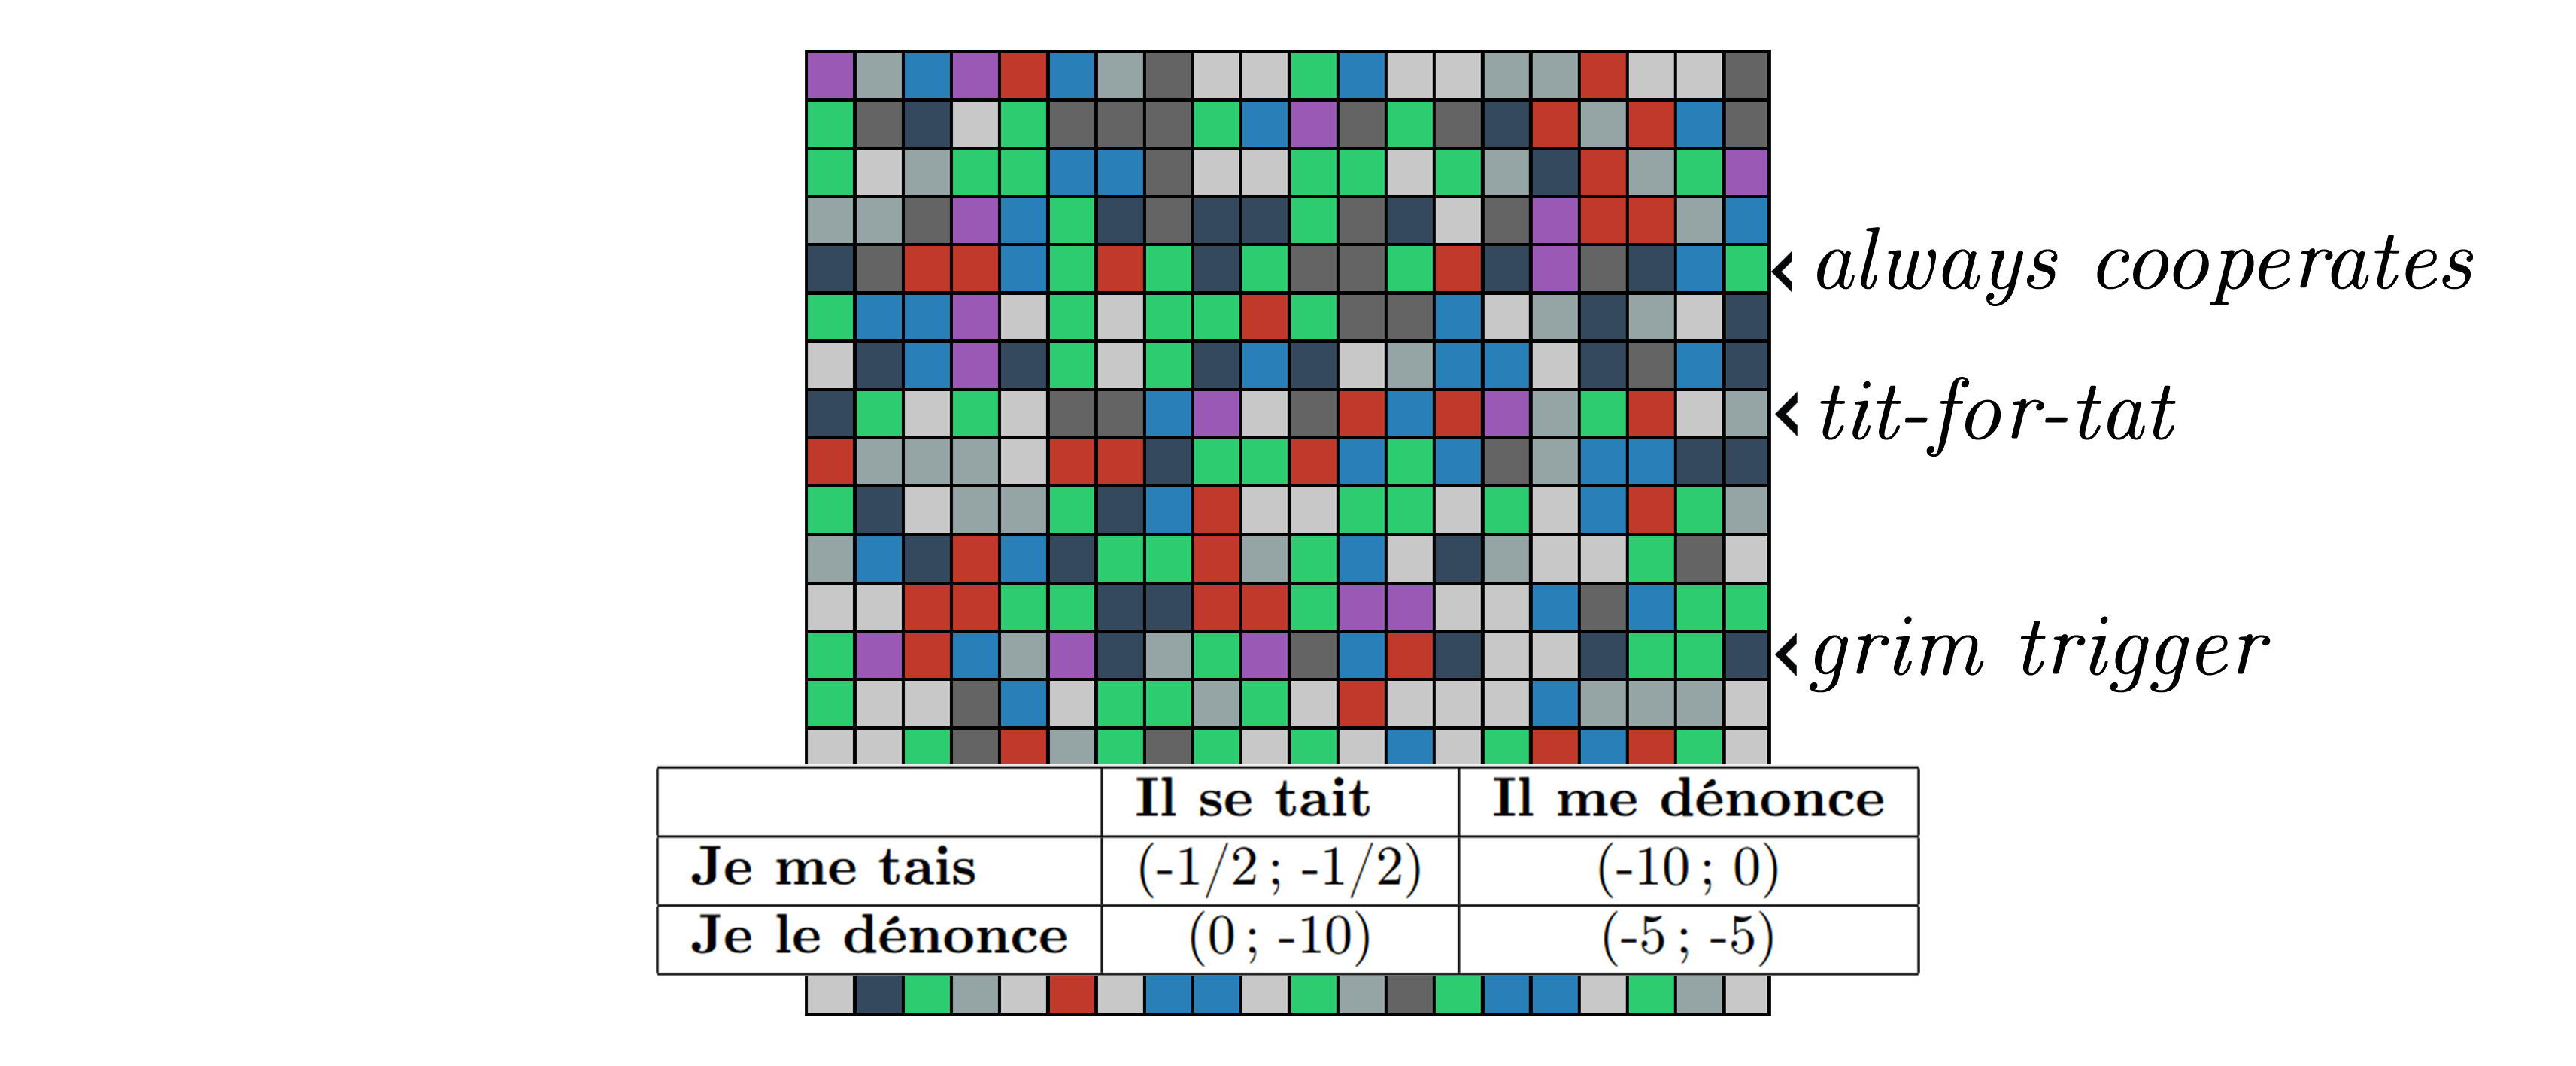
\includegraphics[width=\linewidth]{logo.png}
	\vfill
	\textsc{\class}
	\vspace{1cm}
	
	{\large\today\par}
\end{titlepage}
% End title page

\pagebreak


\section{Abstract}
The purpose of this project is to create a testing environment for the prisoner's dilemma. The prisoner's dilemma is a well known example in the field of game theory, where two players compete in a \textit{zero-sum game} (a game where one player's gains results in losses for the other player). 

In this application, a cellular automaton is modeled after the prisoner's dilemma. A cellular automaton is a grid of colored cells that evolves over time. Each cell has a strategy and plays with each of it's nearest neighbors (one cell apart from our current cell, similar to how the king moves in the game of chess). The user can step forward in time at the press of a button, while data are plotted live on different charts. Girds can also be randomly generated and the payoff of each outcome of the game can be adjusted by means of a payoff matrix.

The prisoner's dilemma cellular automaton is a flexible approach to testing an IPD (iterated prisoner's dilemma) strategy. Strategies can be easily implemented, tested against each other and analysed with charts.


\section{Résumé}
Le but de ce projet est de réaliser un environnement de test pour le dilemme du prisonnier. Le dilemme du prisonnier est un exemple connu dans le domaine de la théorie des jeux, ou deux joueurs s'opposent dans un jeu a somme nulle (un jeu ou les gains d'un des joueurs sont égaux aux pertes de l'autre joueur).

Dans cette application, un automate cellulaire est conçu sur la base du dilemme du prisonnier. Un automate cellulaire est une grille de cellules colorées évoluant au fil du temps. Chaque cellule possède une stratégie et joue avec ses voisins les plus proches (cellules adjacentes à la cellules actuelle, similaire aux mouvements possible d'un roi dans le jeu d'échecs). L'utilisateur peut faire progresser le jeu en appuyant sur un bouton, et les données résultantes sont affichées en temps réel sur des graphiques. Des grilles de cellules peuvent aussi être générées aléatoirement, et la matrice représentant les gains des cellules peut être ajustée.

L'automate cellulaire du dilemme du prisonnier est une solution flexible pour tester des stratégies du DPR (dilemme du prisonnier répété). Diverses stratégies peuvent être ajoutées facilement, testées les unes contre les autres et analysées a l'aide de graphiques.

\pagebreak
\tableofcontents
\pagebreak

% Start document
\section{Introduction}
Ce projet à été réalisé dans le cadre des travaux de diplômes de l'année 2016-2017 du \textbf{C}entre de \textbf{F}ormation \textbf{P}rofessionnelle \textbf{T}echnique en \textbf{I}nformatique dans l'optique d'obtenir un diplôme de Technicien ES.

Durant l'année, nous avons effectués plusieurs travaux sur les automates cellulaires, un sujet auquel je porte un grand intérêt. En lisant différents articles sur internet, il m'est venu l'idée d'un automate cellulaire basé sur le dilemme du prisonnier. Cependant, la majorité de ces articles parviennent de personnes ayant un bagage scientifique en physique, et les démonstrations illustrées dans ces derniers sont réalisés dans des langages axés mathématiques tels que "\textit{R}". 

J'ai comme but de réaliser cet automate cellulaire entièrement en C\# et d'utiliser une bibliothèque permettant d'afficher mes résultats dans un format clair et intuitif à l'utilisateur.

J'ai également comme but d'appliquer les concepts souvent survolés lors des travaux de diplômes tels que le développement piloté par les tests (\textit{test driven development} en anglais) ou encore les patrons de conceptions (\textit{design patterns} en anglais). Ces différents concepts assurent une architecture plus cohérente, et facilite la compréhension pour les personnes extérieures au projet.

\pagebreak
\section{Cahier des charges}
\subsection{Sujet}
Automate cellulaire (voir \href{https://en.wikipedia.org/wiki/Conway's\_Game\_of\_Life}{\textit{Conway's Game of Life}} \cite{GoL}) basé sur le dilemme du prisonnier répété (voir \href{https://en.wikipedia.org/wiki/Prisoner's\_dilemma#The\_iterated\_prisoner.27s\_dilemma}{\textit{Iterated Prisoner's Dilemma}} \cite{DilemmePrisonnier}) et permettant de le simuler.

\subsection{Descriptions}
Le projet étant basé sur deux concepts peu courants, il est nécessaire de les détailler.

\begin{framed}
        \textbf{Automate cellulaire :}
        
        Un automate cellulaire est un modèle constitué d'une grille de cellule changeant d'état à chaque temps $t+1$. Une règle est appliquée à toutes les cellules, habituellement basée sur l'état des voisins de chaque cellule, et permet de faire "évoluer" la grille. L'automate cellulaire le plus connu est probablement \textit{Game of Life} imaginé par John Horton Conway en 1970.

        \vspace{0.5cm}
        \textbf{Dilemme du prisonnier répété : } 
        
        Le dilemme du prisonnier répété est une variante du dilemme du prisonnier. Dans ce jeu, des personnes jouent plusieurs fois au dilemme du prisonnier. 
        
        Dans le dilemme du prisonnier, deux prisonniers ayant commis un crime mineur sont enfermés dans deux cellules différentes, afin de les empêcher de communiquer. Le policier soupçonne les deux accusés d'avoir commis auparavant un crime plus important et souhaite obtenir des aveux concernant ce dernier. Il se présente donc et discute avec chaque prisonnier séparément en leur offrant à chacun deux choix :
        \begin{itemize}
            \item Dénoncer l'autre prisonnier (trahison)
            \item Se taire (coopération)
        \end{itemize}
        
        Il présente donc les résultats des choix suivants :
        
        \begin{itemize}
            \item Si l'un des deux prisonniers dénonce l'autre, il est remis en liberté alors que le second obtient la peine maximale (10 ans)
        
            \item Si les deux se dénoncent entre eux, ils seront condamnés à une peine plus légère (5 ans)

            \item Si les deux refusent de dénoncer l'autre, la peine sera minimale (6 mois), faute d'éléments à charge.
        \end{itemize}
        
        Chaque prisonnier fait donc une \href{https://fr.wikipedia.org/wiki/Matrice\_des\_gains}{\textit{"Matrice des Gains"}} \cite{MatriceGains} pour résoudre ce problème :
        
        \begin{center}
            \begin{tabular}{|l|c|c|}
            \hline
            \textbf{} & \multicolumn{1}{l|}{\textbf{Il se tait}} & \multicolumn{1}{l|}{\textbf{Il me dénonce}} \\ \hline
            \textbf{Je me tais}         & (-1/2 ; -1/2)                            & (-10 ; 0)                                   \\ \hline
            \textbf{Je le dénonce}      & (0 ; -10)                                & (-5 ; -5)                                   \\ \hline
            \end{tabular}
        \end{center}
        
        Chaque prisonnier \textit{devrait} donc comprendre que le choix logique sur une seule itération est de coopérer avec l'autre prisonnier.
\end{framed}

\subsection{But}
Le but du projet est donc de fusionner ces deux concepts et de créer un automate cellulaire permettant de visualiser le dilemme du prisonnier répété. Chaque cellule jouerait une partie du dilemme simultanément avec chacun de ses voisins. Chaque cellule peut adopter une stratégie permettant d'optimiser ses gains. Voici quelques exemples de stratégies :
\begin{framed}
    \begin{description}
        \item[Random (RAND) : ] Fait des actions aléatoires, trahit ou coopère avec 50\% de chance.
        \item[Always Defect (AD) : ] Trahit avec 100\% de chance.
        \item[Always Cooperate (AC) : ] Coopère avec 100\% de chance
        \item[Grim Trigger (GRIM) : ] Stratégie "AC", mais change sa stratégie vers "AD" après trahison.
        \item[\href{http://www.iterated-prisoners-dilemma.net/prisoners-dilemma-strategies.shtml}{\textit{etcetera...}}] \cite{StratIPD}
    \end{description}
\end{framed}

Beaucoup de stratégies peuvent être implémentées pour rendre le jeux intéressant à étudier. Pour cela, des graphiques seront implémentés permettant de récupérer et d'observer les résultats de l'application en temps réel. Les cellules du plateau seront aussi colorées selon leur stratégie ou encore l'historique de leur actions (ex : tendance à trahir $\rightarrow{}$ rouge et tendance à coopérer $\rightarrow{}$ vert).

Voici en exemple, le dilemme du prisonnier sous forme d'automate cellulaire :

\begin{figure}[htp]
    \centering
    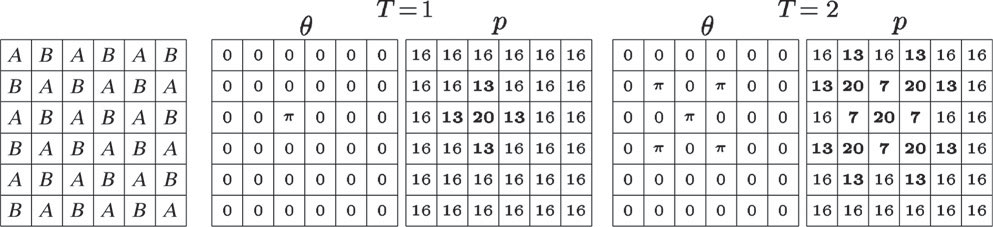
\includegraphics[width=\linewidth]{dilemma.png}
    \caption{Automate cellulaire du dilemme du prisonnier} 
    \textit{source} \cite{DilemmaAutomata}
\end{figure}

\pagebreak{}
\subsection{Spécifications}
Le projet défini dans le cadre suivant :

\begin{itemize}
    \item[] \textbf{Automate cellulaire paramétrable :}
    \begin{itemize}
        \item Nombre de cellules paramétrables.
        \item Stratégies utilisées et proportions de ces dernières sur le plateau paramétrables.
        \item Matrice des gains \cite{MatriceGains} paramétrable.
    \end{itemize}
    \item[] \textbf{Exploitation des résultats :}
    \begin{itemize}
        \item Cellules colorées selon leur stratégie ou historique d'actions.
        \item Divers graphiques (ex : nombre de cellules traîtres par générations)
        \item Possibilité d'utilisation de \href{https://lvcharts.net/}{LiveCharts} \cite{LVCharts}
    \end{itemize}
\end{itemize}

\subsection{Environnement}
Le projet prendra place dans l'environnement suivant :
\begin{itemize}
    \item Ordinateur sous \texttt{Windows 7}
    \item Environnement de développement adapté pour \texttt{C\#}.
\end{itemize}

\subsection{Livrables}
Les documents suivant seront remis à la fin du projet :

\begin{itemize}
    \item Journal de bord (PDF).
    \item Rapport technique (PDF).
    \item Fichier ZIP contenant les sources.
\end{itemize}

\subsection{Reddition}
Voici les dates importantes du projet : 

\begin{framed}
    \begin{itemize}[leftmargin=4cm]
        \item[\textbf{22 Janvier 2017} :] Reddition du cahier des charges.
        \item[\textbf{5 Avril 2017} :] Début du travail
        \item[\textbf{à définir} :] Rendu du poster.
        \item[\textbf{à définir} :] Reddition intermédiaire de la documentation.
        \item[\textbf{12 Juin 2017} :] Reddition finale du projet.
        \item[\textbf{19-20 Juin 2017} :] Présentation orale du projet.
    \end{itemize}
\end{framed}

\begin{sidewaysfigure}[htp]
    \section{Planification provisionnelle}
    \vspace{0.5cm}
    \centering
    \begin{ganttchart}[
    % PARAMETERS
    y unit title=0.5cm,
    y unit chart=0.65cm,
    vgrid,hgrid,
    title height=1,
    title label font=\bfseries\footnotesize,
    bar/.style={fill=BrickRed},
    bar height=0.7,
    group right shift=0,
    group top shift=0.7,
    group height=.3,
    group peaks width={0.2},
    inline]{1}{33}
    /pgf/outer xsep=+0pt,
    canvas/.append style={fill=none},
    link/.append style={thick}]{1}{6}
    % END PARAMETERS
     
        % Labels

        \gantttitle{Travail de Diplôme 2016-2017}{33}\\         
        
        \gantttitle{S1}{3}                    
        \gantttitle{S2}{3}
        \gantttitle{S3}{3}
        \gantttitle{S4}{3}
        \gantttitle{S5}{3}
        \gantttitle{S6}{3}
        \gantttitle{S7}{3} 
        \gantttitle{S8}{3} 
        \gantttitle{S9}{3} 
        \gantttitle{S10}{3} 
        \gantttitle{S11}{3}\\\\
        
        % Content
        \ganttgroup{Vacances de pâques}{5}{9}\\
        \ganttbar[inline=false]{Documentation technique}{1}{4}
        \ganttbar[inline=false]{Documentation technique}{10}{27}\\
        
        \ganttbar[inline=false]{Journal de bord}{1}{4}
        \ganttbar[inline=false]{Journal de bord}{10}{27} \\
        
        \ganttbar[inline=false]{Analyse de existant}{1}{2} \\
        \ganttbar[inline=false]{Planification}{1}{2} \\
        
        \ganttbar[inline=false]{Création du poster}{1}{4}
        \ganttbar[inline=false]{Création du poster}{10}{13} \\
                
        \ganttbar[inline=false]{Conception}{2}{4} 
        \ganttbar[inline=false]{Conception}{10}{15} \\
        
        \ganttbar[inline=false]{Programmation}{4}{4} 
        \ganttbar[inline=false]{Programmation}{10}{27} \\
        
        \ganttbar[inline=false]{Tests unitaires}{4}{4} 
        \ganttbar[inline=false]{Tests unitaires}{10}{27} \\
                
        \ganttbar[inline=false]{Vérifications}{24}{27} \\\\

        \ganttgroup{Soutenances}{30}{32}\\
        \ganttmilestone[inline=false]{Rendu intermédiaire}{15} \\
        \ganttmilestone[inline=false]{Soirée posters}{17} \\
        \ganttmilestone[inline=false]{Rendu abstract}{21} \\
        \ganttmilestone[inline=false]{Rendu final}{27} \\
        \ganttmilestone[inline=false]{Soutenance a blanc}{29} \\
        % Links
        
        
    \end{ganttchart}
    \caption{Diagramme de Gantt}
\end{sidewaysfigure}

\pagebreak
\section{Analyse de l'existant}
Il est nécessaire d'analyser et de comparer différents travaux avant de commencer le développement de notre application. Pour effectuer cette analyse, trois concepts d'automates cellulaires basés sur le dilemme du prisonnier ont étés sélectionnés :

\begin{itemize}
    \item "\textit{A quantum prisoner’s dilemma cellular automaton}" de M. Ramón Alonso-Sanz. \cite{QuantumCellularAutomaton}
    \item "\textit{Prisoner’s dilemma in one-dimensional cellular automata}" de M. Marcelo Alves Pereira \cite{1dCellularAutomaton}
    \item "\textit{The prisoner’s dilemma and the game of life}" de Mme. Katarzyna Zbieć \cite{PDandGoL}
\end{itemize}

\subsection{Projet de M. Ramón Alonso-Sanz}
Le projet de M. Ramón Alonso-Sanz intitulé "\textit{A quantum prisoner’s dilemma cellular automaton}" reprends le dilemme du prisonnier de base, mais y ajoute quelques subtilités :

Le plateau est structuré sous la forme d'un échiquier, chaque cellule a donc quatre alliés et quatre rivaux, comparé à la forme habituelle, qui est d'utiliser les huit voisins de chaque cellules (similaire aux mouvements d'un roi dans le jeu des échecs). Les cellules possèdent des stratégies dites "quantiques" et adaptent aussi leurs stratégies à celle de leurs voisins. Les voisins ayant les meilleures performances sont imités par les autres cellules à l'aide d'une méthode nommé \textit{imitation-of-the best}. Chaque cellule joue aussi avec elle-même en plus de ses rivaux. Ceci permet de prendre en compte ses propres résultats en faisant la moyenne des résultats obtenus entre les parties.

Un mécanisme de mémoire est aussi présent dans le programme de M.Ramon Alonso-Sanz. Ce dernier est de type "Markovien" (voir "chaînes de markov"), un historique complet n'est pas stocké mais les résultats et les choix précédents affectent les choix futurs de chaque cellule.

On compare aussi les stratégies dites "quantiques" aux stratégies classiques pour évaluer l'efficacité de ces dernières. Voici à quoi ressemble le projet de M. Ramón Alonso-Sanz :

\begin{figure}[htp]
    \centering
    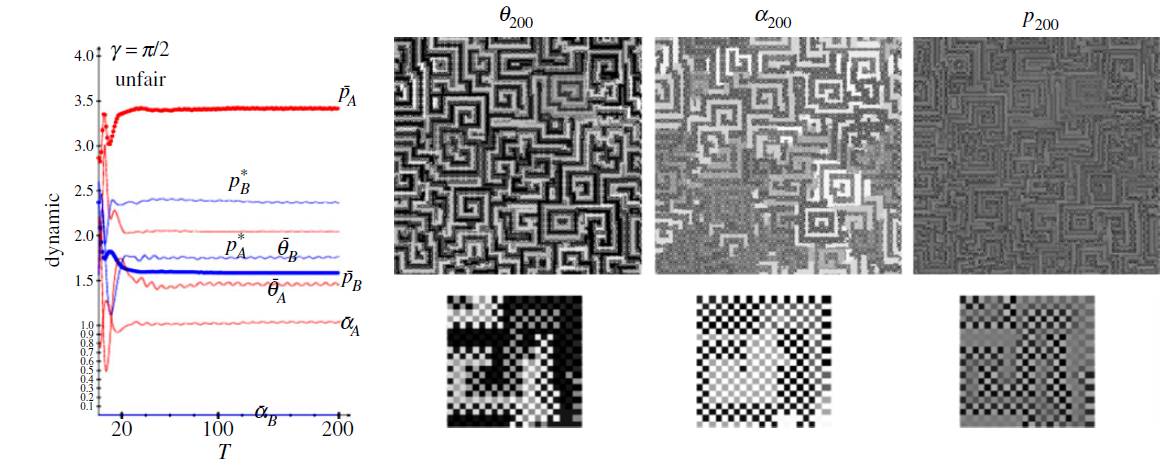
\includegraphics[width=\linewidth]{quantum_automaton.png}
    \caption{Comparaison de stratégies quantiques ($p_A$) et classiques ($p_B$)}
\end{figure}

\pagebreak
\subsection{Projet de M. Marcelo Alves Pereira}
Le projet de M. Marcelo Alves Pereira possède quelques différences avec un automate cellulaire du dilemme du prisonnier standard. En effet, M. Marcelo Alves Pereira allègue que la majorité des automates cellulaires basés sur le dilemme du prisonnier utilisent des structures trop complexes et suggère ainsi une approche plus simple. Ce dernier modélise le dilemme du prisonnier sous la forme d'un treillis à une dimension (tableau à une dimension), mais sa structure comporte quelques subtilités.

La première subtilité est le fait d'empiler ces tableaux à une dimension pour former un tableau en deux dimensions ou chaque position $Y$ du tableau correspond à un temps $T$ d'une partie. Ce système permet d'avoir en \textit{tout temps} un historique complet et visible de la partie actuelle du dilemme du prisonnier. Voici un schéma représentant le fonctionnement de cette approche :

\begin{figure}[htp]
    \centering
    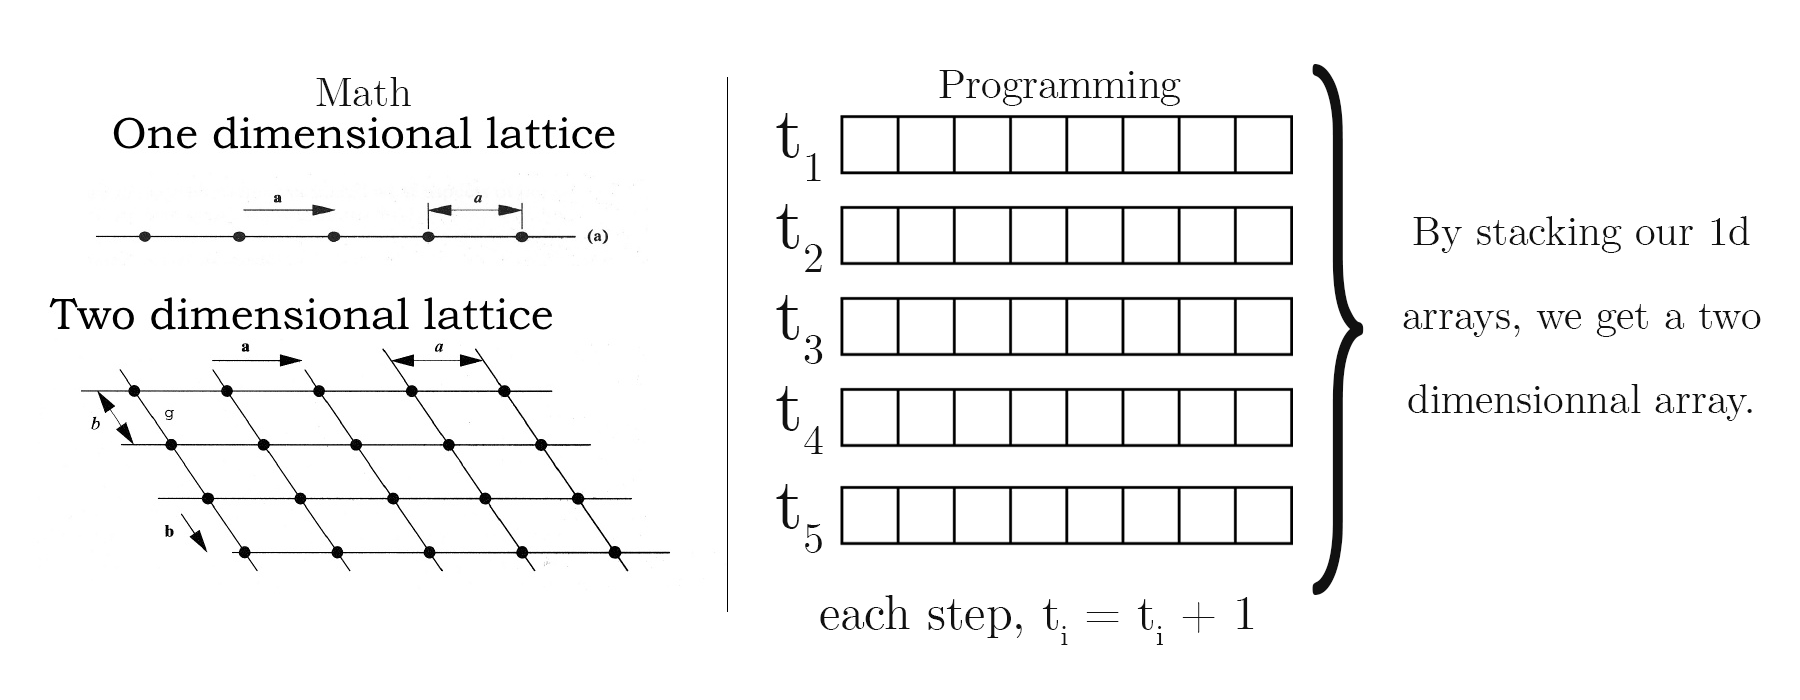
\includegraphics[width=\linewidth]{arrays.png}
    \caption{Utiliser la deuxième dimension d'un tableau pour garder un "historique"}
\end{figure}

La deuxième subtilité est d'utiliser un nombre variable de voisins. En effet, le tableau étant sur un axe unique, on peut représenter le nombre de voisins de chaque cellule simplement par un chiffre $X$ étant pair. Par exemple, pour 6 voisins par cellule, on considère les trois cellules à gauche et a droite de notre cellule actuelle comme nos voisins.

La troisième subtilité est d'utiliser le principe de \textit{self-interaction} (ou "interaction avec soi" en français). Le principe est de "jouer" avec soi-même (la cellule actuelle) pour compenser un manque de joueurs quand le nombre de voisins n'est pas pair (par exemple, sur les bords de la matrice).

Malgré ces subtilités, ce système n'est pas parfait. Les cellules de ce système n'utilisent qu'une seule stratégie : celle du "\textit{tit-for-tat}" (TFT) \cite{StratIPD}. Avec cette stratégie, les cellules commencent dans un état aléatoire et copient la stratégie du voisin ayant obtenu le meilleur score. Ainsi, le jeu devient prévisible; les cellules essaient de maximiser leurs gains de manière "égoïste" et des grappes de cellules trahissant leurs voisins se forment rapidement. Ce système n'est pas une mauvaise représentation du dilemme du prisonnier mais il serait intéressant d'ajouter plus de variations a ce dernier.

\begin{figure}[htp]
    \centering
    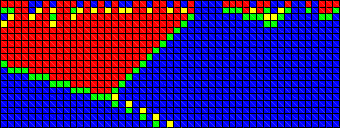
\includegraphics[width=9cm]{defect_cluster.png}
    \caption{Grappe de cellules "traîtres"}
\end{figure}


\pagebreak
\subsection{Projet de Mme. Katarzyna Zbieć}
L'approche de Mme. Katarzyna Zbieć est différente des deux projets précédents. Elle vise à combiner le jeu de la vie de Conway et le dilemme du prisonnier. Les différents principes du jeu de la vie (cellules, états, plateau, etc...) et du dilemme du prisonnier (stratégies, matrice de gains, etc...) sont expliqués en détails et par la suite comparés.

Malheureusement, aucun exemple graphique n'est fourni avec le document. Cependant, ce projet reste le plus proche à celui qui sera développé lors de ce travail de diplôme.

Voici un tableau tiré du document de Mme. Katarzyna Zbieć ainsi que sa traduction française. Ces derniers font ressortir les ressemblances entre la structure du jeu de la vie et celle du dilemme du prisonnier :

\begin{figure}[htp]
    \centering
    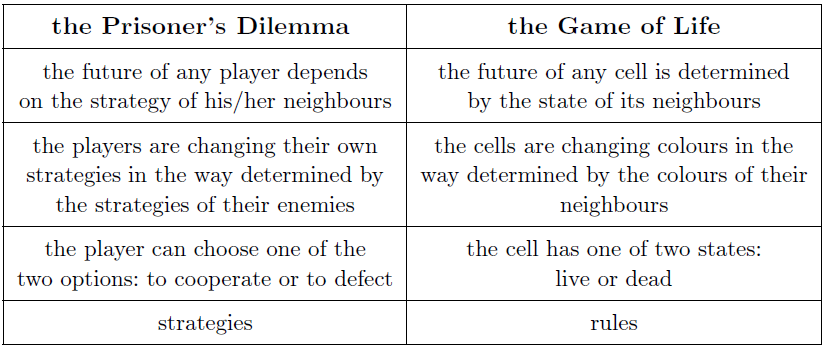
\includegraphics[width=\linewidth - 3cm]{dilemma_gol.png}
    \caption{Comparaison entre le jeu de la vie et le dilemme du prisonnier}
\end{figure}


\begin{table}[htp]
\centering

\begin{tabular}{|c|c|}
\hline
\textbf{Le Dilemme du Prisonnier}                                                                                                     & \textbf{Le Jeu de la Vie}                                                                                     \\ \hline
\begin{tabular}[c]{@{}c@{}}Le futur de chaque joueur dépend\\  de la stratégie de ses voisins\end{tabular}                   & \begin{tabular}[c]{@{}c@{}}Le futur de chaque cellule est déterminé\\ par l'état de ses voisins\end{tabular}          \\ \hline
\begin{tabular}[c]{@{}c@{}}Les joueurs changent leurs stratégies\\ en se basant sur la stratégie de leurs ennemis\end{tabular} & \begin{tabular}[c]{@{}c@{}}Les cellules changent de couleur en\\ fonction de celle de leurs voisins\end{tabular} \\ \hline
\begin{tabular}[c]{@{}c@{}}Le joueur peut choisir deux options :\\ coopérer ou trahir\end{tabular}                            & \begin{tabular}[c]{@{}c@{}}La cellule a deux états :\\ vivante ou morte\end{tabular}                                    \\ \hline
stratégies                                                                                                                    & règles                                                                                                                \\ \hline
\end{tabular}
\caption{Version traduite du tableau des différences entre le \textit{DP} et le \textit{JdlV}}
\end{table}

\subsection{Conclusions tirées de l'analyse}
Des concepts intéressants ressortent de cette analyse, voici des concepts à retenir pour le développement du projet :

\textbf{Système d'historique}\\
\textbf{Stratégies}\\
\textbf{Comparaisons entre stratégies}\\
\textbf{Grille "d'échiquier" pour cellules voisines}\\
\textbf{\textit{Imitation-of-the best}}

\pagebreak
\section{Analyse fonctionnelle}
\subsection{Maquette de l'interface}
Dans cette partie du document, les diverses interfaces graphiques de l'application seront détaillées et expliquées.

\subsubsection{Interactions entre fenêtres}
La fenêtre principale de l'application (en bleu) possède deux modes de fonctionnements : Le mode standard et le mode étendu. C'est depuis cette fenêtre que l'on peut accéder aux divers menus et fenêtres de l'application.

Dans le cas du schéma ci-dessous, on considère la vue principale et la vue étendue comme deux vues différentes. Pour basculer de la vue principale à la vue étendue ou inversement, on actionne un \textit{switch} se trouvant en bas à droite de la fenêtre.

Pour passer de la vue principale (ou étendue) à la fenêtre "à propos", on clique sur le bouton correspondant qui se trouve sur la barre de navigation.

Pour passer de la vue principale (ou étendue) à la fenêtre de paramétrage de la matrice des gains, on clique tout d'abord sur l'onglet "\textit{Settings}" de la barre de navigation, puis sur l'option "\textit{Payoff matrix}" du menu déroulant. Idem pour accéder aux paramètres de génération mais en cliquant sur l'option "\textit{Generate new board}" du menu déroulant.

\vfill
\begin{figure}[htp]
    \centering
    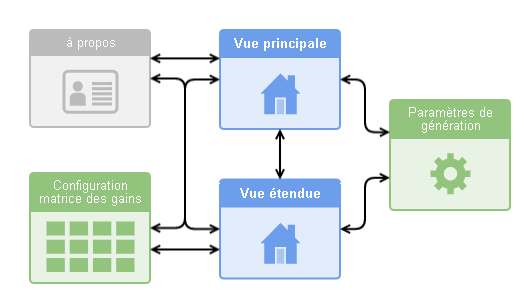
\includegraphics[width=12cm]{interface/app_map.png}
    \caption{Interactions entre fenêtres de l'application}
\end{figure}
\vfill

\pagebreak
\subsubsection{Fenêtre principale}
La fenêtre principale de l'application est composée de plusieurs parties :

\begin{framed}
\begin{description}[align=right, labelwidth=4.25cm]
    \item[\underline{Nom du composant}] \underline{Utilité}
    \item[La grille : ] Composant affichant l'automate cellulaire.
    \item[Paramètres de taille : ] Permet de modifier le nombre de ligne et colonnes de la grille.
    \item[Paramètres de vitesse : ] Modifie la vitesse de \textit{step} en mode d'exécution automatique
    \item[Bouton \textit{step} : ] Passe au temps $t_{i+1}$ de l'automate cellulaire (avance d'un "pas").
    \item[Bouton \textit{start} / \textit{stop} : ] Démarre ou arrête l'exécution automatique de la commande "\textit{step}"
    \item[Bouton \textit{clear} : ] Efface le contenu de la grille.
    \item[Bouton \textit{extended view} : ] Bascule entre la vue principale et la vue étendue.
\end{description}
\end{framed}

L'interface suivante est un croquis et il est possible que des fonctionnalités soient ajoutées à la version finale de l'application.

\vfill
\begin{figure}[htp]
    \centering
    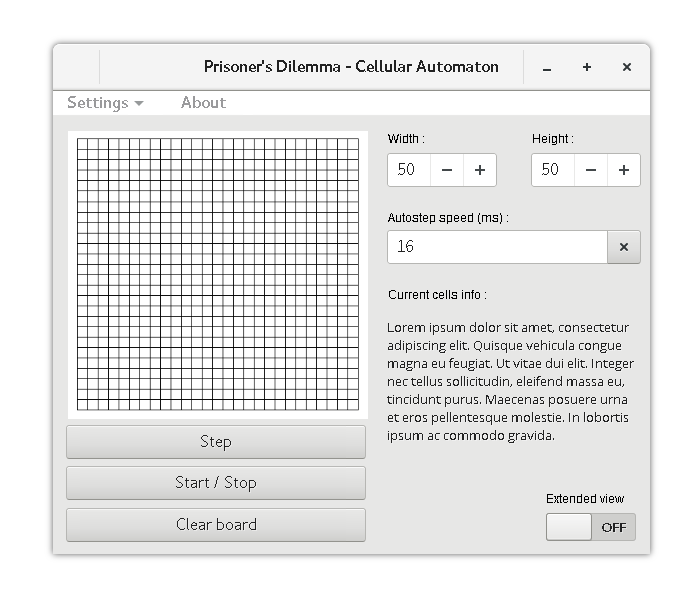
\includegraphics[width=14cm]{interface/mainview.png}
    \caption{Vue principale de l'application}
\end{figure}
\vfill

\pagebreak
\subsubsection{Fenêtre principale (étendue)}
La vue étendue est identique à la vue principale mais possède des graphiques supplémentaires permettant de visualiser plus facilement l'état actuel de l'automate cellulaire.

Voici des exemples de graphiques pouvant être implémentés dans l'application : 

\begin{itemize}
    \item Nombre de cellules "traîtres" par génération.
    \item Nombre de cellules "coopératives" par génération.
    \item Pourcentage de chaque stratégie utilisée.
    \item Stratégie et score maximum associé.
    \item etc...
\end{itemize}

Il est possible de basculer à tout moment de la vue étendue à la vue standard en déactivant le \textit{switch} "\textit{extended view}".

\vfill
\begin{figure}[htp]
    \centering
    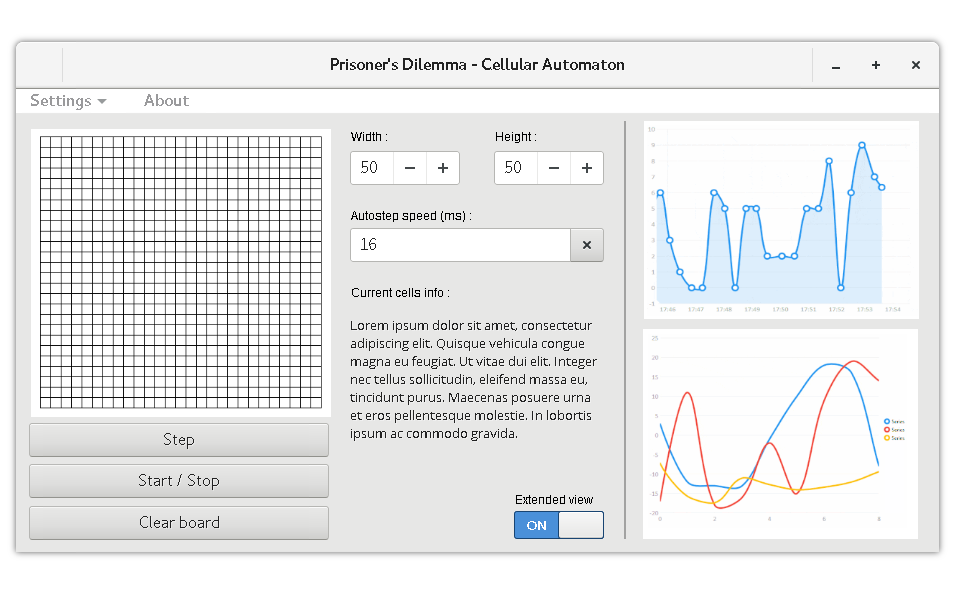
\includegraphics[width=\linewidth]{interface/mainviewextended.png}
    \caption{Fenêtre étendue de l'application}
\end{figure}
\vfill

\pagebreak
\subsubsection{Fenêtre principale, paramètres et "à propos"}
Sur la fenêtre principale (ou étendue), une barre de navigation est présente en haut de page. Grâce à cette dernière, on peut accéder à un menu déroulant des paramètres de l'application (figure inférieure) et à la fenêtre à propos (figure supérieure).

Depuis le menu déroulant des paramètres, en cliquant sur le bouton "\textit{Payoff matix}", on accède aux paramètres de la matrice de gains (voir "Matrice des gains"). En cliquant sur "\textit{Generate new board}" : on accède aux paramètres de la génération d'un nouveau plateau (voir "Paramètres de génération").

\vfill
\begin{figure}[htp]
    \centering
    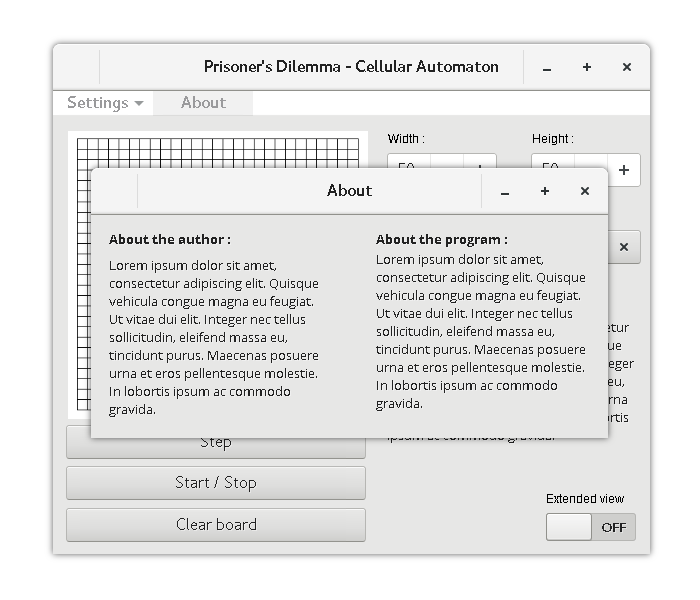
\includegraphics[width=10cm]{interface/mainviewabout.png}
    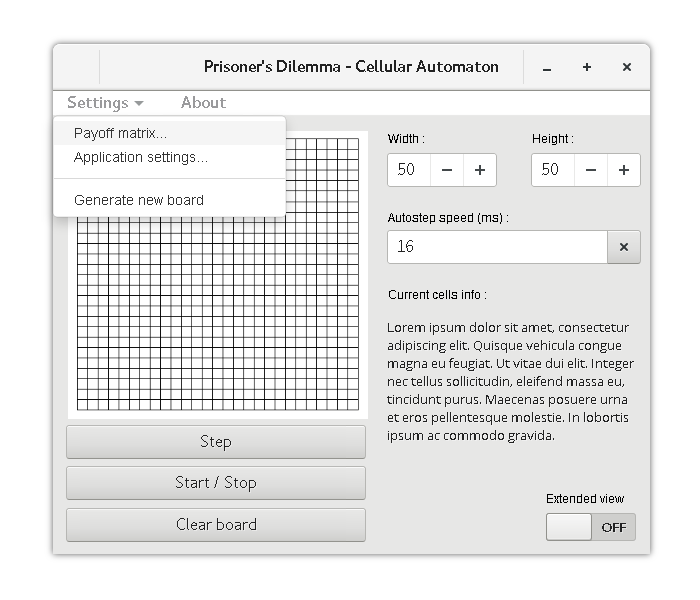
\includegraphics[width=10cm]{interface/mainviewsettings.png}
    \caption{Fenêtre "à propos" et accès aux paramètres de l'application}
\end{figure}
\vfill

\pagebreak
\subsubsection{Matrice des gains}
Sur la fenêtre des paramètres de la matrice des gains, on peut modifier différentes valeurs qui par la suite affecteront le comportement des cellules du plateau. Les paramètres présents sur la fenêtre correspondent aux quatre résultats pouvant être obtenus lors d'une partie du dilemme du prisonnier.

Les choix sont les suivants : 

\begin{itemize}
    \item \textit{Reward payoff} ($R$)
    \item \textit{Sucker's payoff} ($S$)
    \item \textit{Temptation's payoff} ($T$) ou couramment appelé \textit{Cheat's payoff} ($C$) 
    \item \textit{Punishment's payoff} ($P$)
\end{itemize}

On résume donc les valeurs de la matrice par les lettres $R$ pour deux joueurs qui coopèrent, $S$ pour le joueur s'étant fait trahir, $T$ ou $C$ pour le joueur ayant trahi et $P$ pour les deux joueurs s'étant trahi.

On ne peut pas insérer n'importe quelles valeurs dans la matrice des gains. Les règles concernant les valeurs de la matrice sont les suivante :

\begin{framed}
    \centering
    $T < R < P < S$\\
    $2R < T + S$
\end{framed}

En cliquant sur le bouton "\textit{OK}" se trouvant en bas de la fenêtre, on applique les modifications à la matrice des gains et on retourne sur la vue principale (ou étendue). Notez que le bouton "\textit{OK}" de la page sera uniquement activé si les deux conditions citées précédemment sont respectées.

\vfill
\begin{figure}[htp]
    \centering
    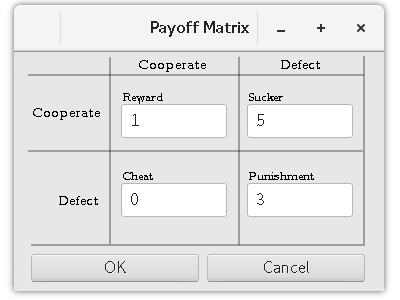
\includegraphics[width=10cm]{interface/payoffmatrix.png}
    \caption{Configuration de la matrice des gains de l'application}
\end{figure}
\vfill

\pagebreak
\subsubsection{Paramètres de génération}
La fenêtre "Paramètres de génération" donne la possibilité à l'utilisateur de générer un plateau de cellules avec un répartition aléatoire mais proportionnelle des stratégies.

On peut sélectionner les stratégies différentes à répartir sur le plateau à l'aide d'un champ texte. Voici un exemple correct de répartition des stratégies :

\begin{framed}
\begin{description}[align=left, labelwidth=4.35cm]
    \item[Random (RAND)] : 15\%
    \item[Always Defect (AD)] : 15\%
    \item[Always Cooperate (AC)] : 35\%
    \item[Grim Trigger (GRIM)] : 35\%
    \vspace{0.1cm}
    \hrule
    \vspace{0.1cm}
    \item[Total] : 100\%
\end{description}
\end{framed}

Le pourcentage total des stratégies sélectionnées doit impérativement être égal à 100\%. Si ce n'est pas le cas, l'interface ne permettra pas à l'utilisateur de continuer (voir "Paramètres de génération, contrôles).

\vfill
\begin{figure}[htp]
    \centering
    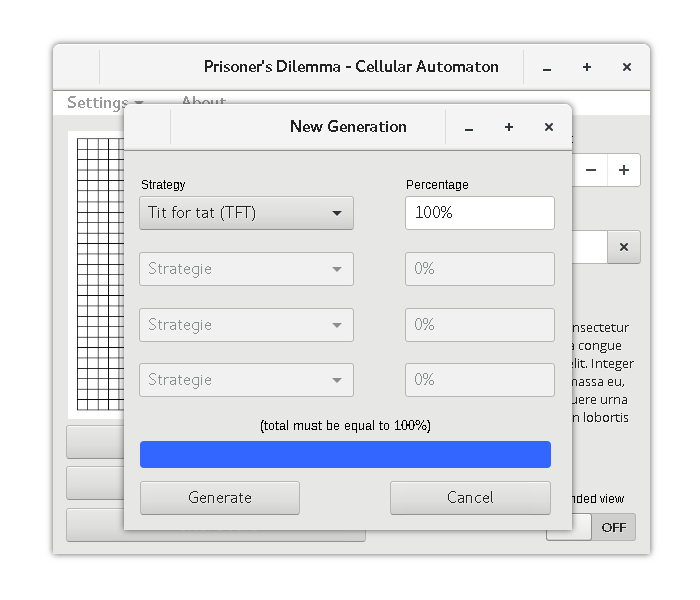
\includegraphics[width=12cm]{interface/generationsettings.png}
    \caption{Répartition aléatoire de cellules}
\end{figure}
\vfill

\pagebreak
\subsubsection{Paramètres de génération, contrôles}
Cette vue est ici pour démontrer les contrôles de la page "Paramètres de génération" empêchant les utilisateurs d'entrer des valeurs incorrectes. Notez que la barre de progression se trouvant en bas de la page est inférieure à 100\%, empêchant ainsi l'accès à la génération du nouveau plateau.

\vfill
\begin{figure}[htp]
    \centering
    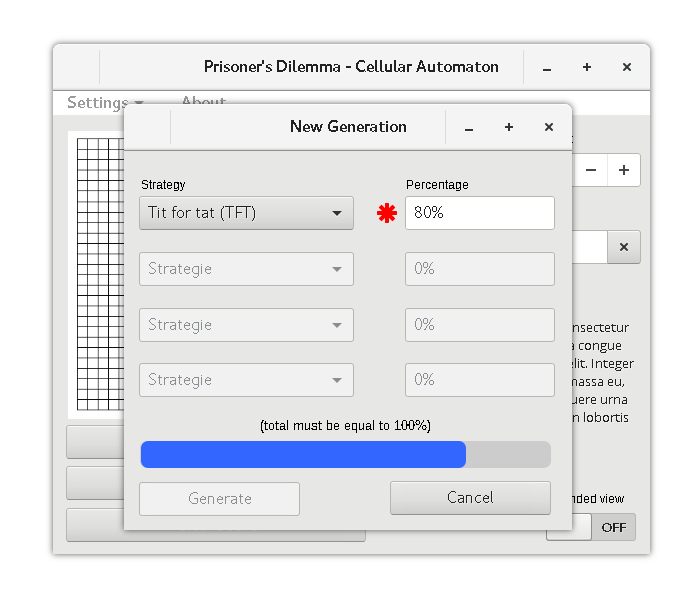
\includegraphics[width=12cm]{interface/generationsettingsinvalid.png}
    \caption{Gestion des erreurs sur la génération aléatoire de cellules}
\end{figure}
\vfill
\pagebreak

\subsection{Technologies utilisées}
\subsubsection{\textit{LiveCharts}}
\textit{LiveCharts} est une bibliothèque C\# permettant d'inclure des graphiques dynamiques dans des environnements \textit{WPF} et \textit{WinForms}. La bibliothèque permet l'utilisation de différents graphiques :

\begin{itemize}
    \item \textit{Cartesian charts} (Tableaux cartésiens)
    \item \textit{Pie charts} (Camemberts)
    \item \textit{Solid gauges} (Jauges)
    \item \textit{Angular gauges} (Jauges angulaire)
    \item \textit{Heatmaps \& Geo maps} (Cartes)
\end{itemize}

Dans le cadre de ce projet, des tableaux cartésiens et des camemberts seront principalement utilisés pour représenter les données.

\vspace{0.5cm}
\begin{figure}[htp]
    \centering
    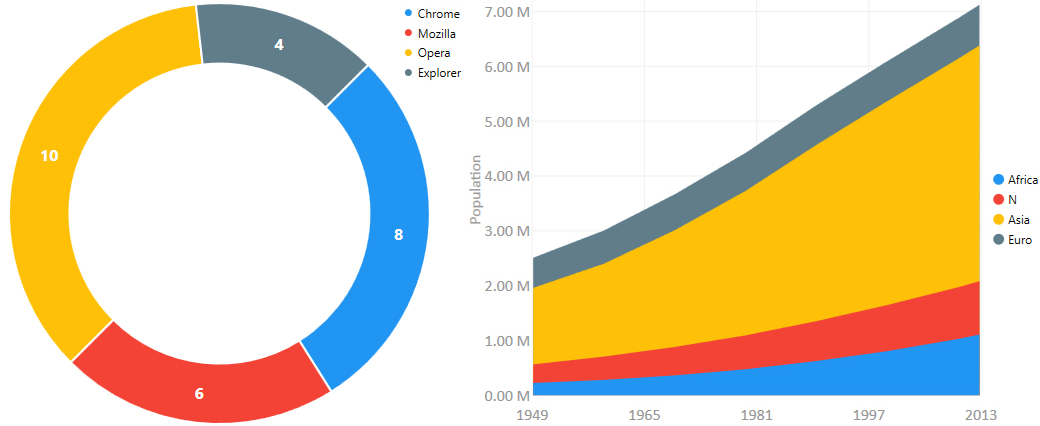
\includegraphics[width=\linewidth]{charts.png}
    \caption{Exemples de graphiques réalisés avec \textit{LiveChars}}
\end{figure}

\subsubsection{Tests unitaires}
Les tests unitaires sont nécessaire pour vérifier le bon fonctionnement des différentes fonctions d'un projet. Traditionnellement, les tests sont réalisés avant le développement des fonctions. On appelle ce principe du "développement piloté par des tests" (ou \textit{test driven developpement} en anglais). 

Les tests unitaires facilitent différents aspects de la programmation : 
\begin{itemize}
    \item Faciliter le \textit{debugging}
    \item Faciliter la maintenance
    \item Faciliter la rédaction de documentation
\end{itemize}

Les tests unitaires sont considérés comme de bonnes partiques lors du développement d'une application.

Dans le cadre de ce projet, toutes les fonctions du modèle seront testées à l'aide de tests unitaires.

\pagebreak
\subsubsection{\textit{Design patterns}}
Les \textit{design patterns} (ou "patrons de conception") en français sont des solutions générales que l'on peut appliquer a un projet lors de sa conception. Un \textit{design pattern} est reconnu comme une bonne pratique et est encouragé lors de la conception d'un logiciel.

Dans le cadre de l'automate cellulaire, le \textit{design pattern} "\textit{Strategy}" sera utilisé pour le mécanisme de stratégies des cellules. Ce design pattern permet de déléguer une méthode de notre classe à une classe spécialisée. Dans notre cas, la cellule délègue le choix de sa prochaine action à sa stratégie actuelle.

Voici un exemple UML du \textit{design pattern} "\textit{Strategy}" :

\begin{figure}[htp]
    \centering
    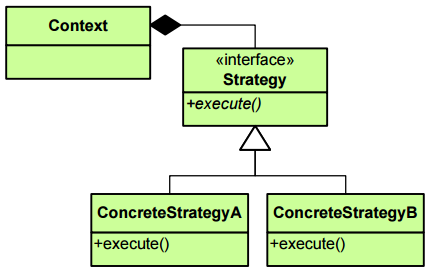
\includegraphics[width=8cm]{strategy.png}
    \caption{Patron de conception "\textit{Strategy}"}
\end{figure}

\subsubsection{Sérialisation}
La stérilisation permet d'enregistrer l'état de la mémoire d'une application dans un format spécifique. Dans le cadre de mon projet, la sérialisation sera implémentée au format "\textit{.xml}". Le processus de récupération de ces données se nomme dé-sérialisation, et consiste a parcourir le fichier de données externe et de mettre en mémoire les différentes informations récupérées.

\vfill
\begin{figure}[htp]
    \centering
    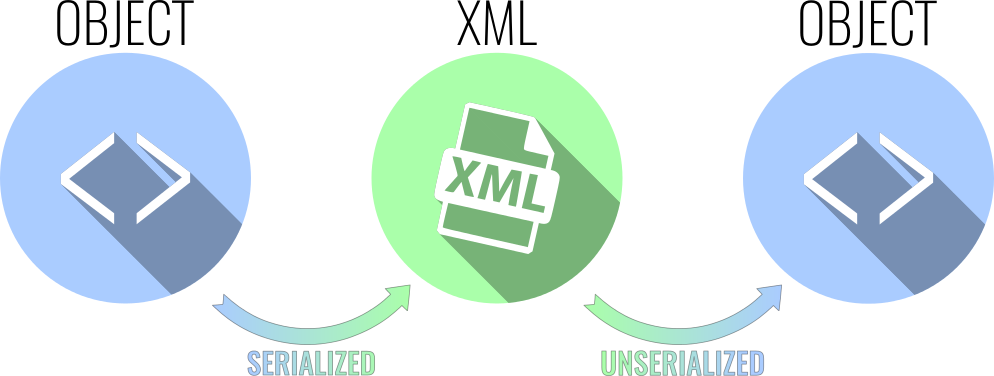
\includegraphics[width=\linewidth - 2cm]{serialization.png}
    \caption{Schéma de sérialisation "\textit{.xml}"}
\end{figure}
\vfill

\pagebreak
\subsection{Stratégies}
Les joueurs du dilemme du prisonier utilisent de diverses stratégies\cite{StratIPD}\cite{StratIPD2} dans le but d'obtenir le meilleur score. Dans ce chapitre, les différentes stratégies adoptées par les cellules seront décrites en détail. On peut classer les stratégies en plusieurs groupes :
\begin{itemize}
    \item Les stratégies originales (ex : \textit{always cooperate}, \textit{grim trigger}, etc...)
    \item \textit{Tit-for-tat} et ses variantes. (ex : \textit{tit-for-tat}, \textit{reverse tit-for-tat}, etc...)
    \item Les stratégies de groupe (ex : \textit{handshake}, \textit{fortress}, etc...)
\end{itemize}

\subsubsection{\textit{Tit-for-tat}}
\textit{Tit-for-tat} est considéré comme la stratégie la plus simple ayant les meilleurs résultats\cite{TFT}. Le nom \textit{Tit-for-tat} implique une idée similaire à celle de "oeil pour oeil dent pour dent". Son fonctionnement est le suivant : on commence tout d'abord par coopérer, puis on observe le score de chacun de nos voisins. On copie par la suite la dernière action du voisin ayant obtenu le meilleur score.

Cette stratégie se retrouve couramment dans une situation de "\textit{deadlock}", c'est-à-dire, une situation on l'on ne peut plus revenir à la coopération et ou trahir reste la seule bonne option.

\subsubsection{\textit{Tit-for-two-tats}}
\textit{Tit-for-two-tats} est une variante de \textit{Tit-for-tat} ou on copie l'action du meilleur voisin uniquement si il fait deux fois la même action d'affilée. Si un voisin ne joue pas deux fois la même action d'affilée, on reste sur notre dernière action.

\subsubsection{\textit{Reverse tit-for-tat}}
\textit{Reverse tit-for-tat} est une variante de \textit{Tit-for-tat}. Comme son nom l'indique, cette stratégie effectue les actions inverses de \textit{Tit-for-tat}. Le joueur avec cette stratégie commence par trahir, puis il regarde la dernière action de son meilleur voisin et joue l'inverse au prochain tour.

\subsubsection{\textit{Always cooperate}}
Comme son nom l'indique, un joueur avec cette stratégie \textit{coopère} toujours.

\subsubsection{\textit{Always defect}}
Comme son nom l'indique, un joueur avec cette stratégie \textit{trahit} toujours.

\subsubsection{\textit{Random}}
Comme son nom l'indique, un joueur avec cette stratégie joue de manière \textit{aléatoire}. On pourrait comparer cette stratégie avec un joueur jouant a pile ou face à chaque tour pour déterminer sa prochaine action.

\subsubsection{\textit{Blinker}}
Le mot \textit{blinker} venant de l'anglais peut être traduit littéralement par "clignotant", illustrant le comportement de cette stratégie. Cette stratégie commence par coopérer, puis alterne entre trahison et coopération.

\subsubsection{\textit{Grim trigger}}
La stratégie \textit{grim trigger} est une stratégie que l'on peut dire "rancunière". Le joueur coopère tout le temps à la manière \textit{always cooperate} jusqu'à qu'un joueur le trahisse. Après avoir été trahit, le joueur adopte une stratégie \textit{always defect} et trahit de manière permanente.

\subsubsection{\textit{Handshake}}
\textit{Handshake} est la plus simple des stratégies de groupe. Elle consiste a identifier les voisins utilisant aussi la stratégie \textit{Handshake}. Elle commence par "trahir, coopérer", si l'un de ses voisins effectue cette séquence, on coopère toujours, sinon on trahit toujours.


\subsubsection{\textit{Fortress}}
\textit{Fortress} est une stratégie de groupe visant a reconnaître les voisins utilisant aussi la stratégie \textit{Fortress}. Elle est similaire à la stratégie \textit{Handshake}. Elle commence par une séquence "trahir, trahir, coopérer", si l'un de ces voisins effectue cette même séquence, on la considère comme un "allié". Après avoir trouvé un "allié", on coopère jusqu'à la fin. Si on ne trouve pas "d'allié", on continue la séquence "trahir, trahir, coopérer".

\subsubsection{\textit{Southampton Group Strategy} (SGS)}
Cette stratégie est similaire a \textit{Fortress} et \textit{Handshake}; elle essaie d'identifier des voisins ayant la même stratégie avant d'effectuer une série d'action apportant un nombre maximal de points. 

Dans le cas de \textit{southampton group strategy}, elle commence par jouer une séquence de 5 à 10 mouvements prédéfinis au début de la partie. Après avoir reconnu d'autres cellules utilisant \textit{southampton group strategy}, les cellules élisent un "maître" et le reste adoptent le comportement "d'esclave". La cellule "maître" trahit tout le temps et les cellules voisines "esclaves" coopèrent pour assurer le maximum de points au "maitre". Si une cellule \textit{southampton group strategy} n'arrive pas a identifier des "aliés", elle trahit le reste de la partie.

\subsubsection{\textit{Pavlov}}
\textit{Pavlov} est une stratégie dite \textit{heuristique} ou \textit{rule-based} en anglais. Elle consiste a identifier la stratégie de ses voisins à l'aide de règles prédéfinies. Les stratégies des voisins sont classées dans quatre groupes :
\begin{itemize}
    \item \textit{Cooperative} (coopératif)
    \item \textit{Always defects} (trahit toujours)
    \item \textit{Tit-for-tat}
    \item \textit{Random} (aléatoire)
\end{itemize}

Les six premiers tours de la partie sont consacrés à l'analyse des voisins, pendent cette période, \textit{Pavlov} joue de manière identique à \textit{Tit-for-tat}. Si l'adversaire ne commence pas a trahir dans ces tours, on l'identifie en tant que coopératif, \textit{Pavlov} adopte donc une stratégie \textit{Tit-for-tat}. Si l'adversaire trahit plus de quatre fois sur six, il est identifié en tant que \textit{traitre} (trahit toujours) et \textit{Pavlov} adopte une stratégie \textit{always defect}. Si un voisins trahit exactement trois fois sur six, elle est identifiée en tant que \textit{tit-for-tat} et \textit{Pavlov} adopte donc une stratégie \textit{tit-for-two-tats} pour essayer de coopérer avec \textit{tit-for-tat}. Si un adversaire ne rentre pas dans ces catégories, on la classifie en tant que \textit{random} (aléatoire) et \textit{Pavlov} joue \textit{always defect}. Les voisins peuvent cependant changer leurs actions, pour contrer ce mécanisme, \textit{Pavlov} ré-évalue ses voisins chaque six tours.

\pagebreak
\section{Analyse organique}
\subsection{Diagramme de classe}

\begin{figure}[htp]
    \centering
    \begin{tikzpicture}[thick,scale=0.85, every node/.style={transform shape}]
        % BEGIN Move Enum
        \umlclass[x=0,y=7,type=enumeration]{Move}
        {
        Literals :\\
            - Cooperate\\
            - Defect
        }
        {}
        % END Move Enum
    
        % BEGIN ColorMode Enum
        \umlclass[x=4,y=7,type=enumeration]{ColorMode}
        {
        Literals :\\
            - Strategy\\
            - Playing
        }
        {}
        % END ColorMode Enum
        
        % BEGIN WrapMode Enum
        \umlclass[x=8,y=7,type=enumeration]{WrapMode}
        {
        Literals :\\
            - Default\\
            - Torus
        }
        {}
        % END WrapMode Enum
    
        % BEGIN Cell class
        \umlclass[x=-6,y=-1]{Cell}
        % Fields
        {
            - \_x : int\\
            - \_y : int\\
            - \_width : int\\
            - \_height : int\\
            - \_score : int\\
            - \_strategy : Strategy\\
            - \_color : Color\\
            - \_neighbors : List<Cell>\\
            - \_choice : Move\\
            - \_history : Stack<Move>
        }
        % Methods
        {
            + step() : void\\
            + draw() : void\\
            + chooseNextMove() : void\\
            + updateLastMove() : void\\
            + updateStrategy(Strategy strat) : void\\
            + onClick(int x, int y, Strategy strat) : void\\
            + setColorFromMove() : void\\
            + setColorFromStrategy() : void\\
            + GetSchema() : XmlSchema\\
            + ReadXml(XmlReader reader) : void\\
            + WriteXml(XmlWriter writer) : void\\
            + implicit operator : Rectangle()
        }
        % END Cell class
        
        % BEGIN Grid class
        \umlclass[x=4,y=-1]{Grid}
        % Fields
        {
            - \_cells : Cell[,]\\
            - \_width : int\\
            - \_height : int\\
            - \_nbCols : int\\
            - \_nbLines : int\\
            - \_payoffMatrix : PayoffMatrix\\
            - \_colorMode : ColorMode
        }
        % Methods
        {
            + step() : void\\
            + draw() : void\\
            + generate(Dictionary<Strategy, int> percentages)\\
            + getCell(int x, int y) : Cell\\
            + onClick(int x, int y, Strategy strat) : void\\
            + setStrategy(int x, int y, Strategy strat) : void\\
            + setColorMode(ColorMode mode) : void\\
            + findCountOfStrategy(Strategy strategy) : int\\
            + findAvgScoreOfStrategy(Strategy strategy) : double\\
            - getPointClampedInGrid(int x, int y) : Point\\
            - findCellNeighbors(Cell cell) : List<Cell>\\
            - setColorFromStrategy() : void\\
            - setColorFromMove() : void
        }
        % END Grid class
        
        
        % BEGIN PayoffMatrix class
        \umlclass[x=-6,y=7]{PayoffMatrix}
        % Fields
        {
        - \_reward : int\\
        - \_sucker : int\\
        - \_temptation : int\\
        - \_punishment : int
        }
        % Methods
        {
            + isValid() : bool\\
            + \underline{isValid(int t, int r, int p, int s) : bool}\\
            + returnPayoff(Move p1, Move p2) : int
        }
        % END PayoffMatrix class
        
        % BEGIN Strategy interface
        \umlclass[x=-6,y=-8, type=abstract]{Strategy}
        % Fields
        {}
        % Methods
        {
            + chooseMove(cell : Cell, neighbors : List<Cell>) : void\\
            + getColor() : Color\\
            + ToString() : String
        }
        % END Strategy interface
    
        \umlsimpleclass[x=-8, y=-10]{TFT}
        \umlsimpleclass[x=-6, y=-10]{RAND}
        \umlsimpleclass[x=-4, y=-10]{GRIM}
        \umlsimpleclass[x=1, y=-8]{IXmlSerializable}
        
        % Links
        \umlassoc[]{Move}{Cell}
        \umlassoc[]{ColorMode}{Grid}
        \umlassoc[]{WrapMode}{Grid}
        \umlassoc[geometry=|-|, weight=0.4]{Move}{PayoffMatrix}
        \umlassoc{Cell}{PayoffMatrix}
        \umlcompo{Grid}{Cell}
        \umlaggreg{Cell}{Strategy}
        \umlinherit{TFT}{Strategy}
        \umlinherit{RAND}{Strategy}
        \umlinherit{GRIM}{Strategy}
        \umlreal{Cell}{IXmlSerializable}

        % Notes
    \umlnote[x=1, y=-10]{Strategy}{cf. the "\textit{Strategy}" design pattern}
    
    \end{tikzpicture}
    \caption{Modèle UML de l'automate cellulaire du dilemme du prisonnier}
\end{figure}

\pagebreak
\subsection{Conventions de codage}
Voici les conventions de codage respectées par toutes les classes de l'application.

\subsubsection{En-têtes}
Chaque classe de l'application possède une en-tête. Dans cette en tête, on résume la fonction de la classe, son auteur ainsi que sa date de création.

\begin{lstlisting}
/*
    Class           :   Name.cs
    Description     :   
    Author          :   SEEMULLER Julien
    Date            :   DD.MM.YYYY
*/
\end{lstlisting}

\subsubsection{Commentaires}
Chaque fonction de l'application est commentée. Le commentaire possède une courte explication de l'utilité de la fonction ainsi qu'une explication des paramètres si il y en a.

\begin{lstlisting}
/// <summary>
/// Use of function
/// </summary>
/// <param name="param1">Use of the first parameter</param>
/// <param name="param2">Use of the second parameter</param>
/// <param name="param3">etc...</param>
\end{lstlisting}

\subsubsection{Structure d'une classe}
Chaque classe est découpée en six parties. En haut de classe se trouve l'en-tête, suivi par les \textit{usings} et finalement suivi par le contenu de la classe. La classe est séparée en quatre parties à l'aide de régions (\texttt{\#region}): les champs, les propriétés, les constructeurs et les méthodes.

Voici un exemple de structure de code :

\begin{lstlisting}
/* Header  */

using System;
using System.Collections.Generic;
[...]

public class myClass {
    #region fields
    #endregion
    
    #region properties
    #endregion
    
    #region constructors
    #endregion
    
    #region methods
    #endregion
}
\end{lstlisting}

\pagebreak
\subsection{Classes de l'automate cellulaire}
Voici les différentes classes liés au fonctionnement de l'automate cellulaire :
\begin{itemize}
    \item Classe \texttt{Cell}
    \item Classe \texttt{Grid}
    \item Classe \texttt{PayoffMatrix}
    \item Classe abstraite \texttt{Strategy}
    \item Énumérations \texttt{Move}, \texttt{ColorMode} et \texttt{WrapMode}
\end{itemize}

Dans ce chapitre vous trouverez le résumé détaillé du fonctionnement et de l'utilité de chacune de ces classes.

\subsubsection{Classe \texttt{Cell}}
La classe \texttt{Cell} est l'élément principal peuplant la grille de l'automate cellulaire. Voici les champs de la classe cellule ainsi qu'une courte description :  

\vspace{0.25cm}
\begin{description}[labelwidth=2.50cm]
    \small
    \item[\textbf{\textsc{Champ}}] \textbf{\textsc{Description}}
    \vspace{0.1cm}
    \hrule{}
    \item[\texttt{x}]             :  Numéro de la colonne ou se trouve la cellule.
    \item[\texttt{y}]             :  Numéro de la ligne ou se trouve la cellule.
    \item[\texttt{width}]         :  Largeur de la cellule en \textit{pixels}.
    \item[\texttt{height}]        :  Hauteur de la cellule en \textit{pixels}.
    \item[\texttt{score}]         :  Nombre de jours en prison de la cellule au tour actuel.
    \item[\texttt{strategy}]      :  Stratégie actuelle de la cellule. Determine les actions de la cellule.
    \item[\texttt{color}]         :  Couleur actuelle de la cellule.
    \item[\texttt{neighbors}]     :  Références vers les cellules voisines de la cellule.
    \item[\texttt{payoffMatrix}]  :  Référence vers la matrice des gains utilisée pour calculer le score de la cellule.
    \item[\texttt{choice}]      :  Prochaine action de la cellule (voir Énumération \texttt{Move}).
    \item[\texttt{history}]       :  Liste de toutes les actions de la cellule.
\end{description}
\hrule{}
\vspace{0.5cm}

Suivant la philosophie \textit{tell don't ask}, la logique ainsi que les données sont stockées à l'intérieur de la cellule. Chaque cellule est "responsable" du bon déroulement des méthodes appelées par les autres composants. La cellule a donc connaissance de tous ses voisins ainsi que la matrice de gains à l'aide de références vers ces derniers. Voici les méthodes de la classe cellule : 

\vspace{0.25cm}
\begin{description}[labelwidth=3.85cm]
    \small
    \item[\textbf{\textsc{Méthode}}] \textbf{\textsc{Description}}
    \vspace{0.1cm}
    \hrule{}
    \item[\texttt{step()}]                  :   Joue une partie avec les voisins de la cellule en utilisant le choix actuel.
    \item[\texttt{chooseNextMove()}]        :   Choisit le prochain choix de la cellule (trahir ou coopérer) grâce à sa stratégie.
    \item[\texttt{updateLastMove()}]        :   Ajoute la dernière action effectuée à l'historique 
    \item[\texttt{draw()}]                  :   Dessine la cellule sur l'élément graphique passé en paramètre.
    \item[\texttt{setColorFromMove()}]      :   Change la couleur de la cellule selon ses actions (ex: trahir = rouge)
    \item[\texttt{setColorFromStrategy()}]  :   Change la couleur de la cellule selon sa stratégie (ex: \textit{AC} = vert)
    \item[\texttt{updateStrategy()}]        :   Remplace la stratégie de la cellule avec celle passée en paramètre.
    \item[\texttt{Rectangle()}]             :   Précédé par \texttt{implicit operator} $\rightarrow$ conversion implicite de cellule en rectangle.
    \item[\texttt{onClick()}]               :   Change la stratégie avec celle passée en paramètre.
    \item[\texttt{GetSchema()}]             :   Inutilisé. Imposé par l'interface IXmlSerializable.
    \item[\texttt{ReadXml()}]               :   Lit le contenu d'une cellule depuis un fichier XML. Imposé par IXmlSerializable.
    \item[\texttt{WriteXml()}]              :   Écrit le contenu d'une cellule dans un fichier XML. Imposé par IXmlSerializable.
\end{description}
\hrule{}
\vspace{0.5cm}
\pagebreak

\subsubsection{Analyse des méthodes de la classe \texttt{Cell}}
\textbf{Méthode "step()"}\\
La méthode \texttt{step()} est la fonction principale de \texttt{Cell}. Elle permet de jouer une partie du dilemme du prisonnier avec ses voisins. On peut résumer une partie du dilemme du prisonnier par l'interaction entre deux actions (énumération \texttt{Move}) et la récompense qu'elles apportent. Pour obtenir ses gains, elle se réfère donc à la matrice des gains actuelle à l'aide de la méthode \texttt{returnPayoff()} (voir classe \texttt{PayoffMatrix}). 

Après avoir récupéré le score de chacune des parties, on récupère le meilleur score (score minimum) de ces dernières comme score représentatif. D'autres alternatives comme une moyenne du score ou encore une médiane \cite{Median} ont été testées mais elles ne permettaient pas une bonne représentation du score et faussaient les calculs de certaines stratégies.

Voici a quoi ressemble la méthode \texttt{step()} de la classe \texttt{Cell} :
\begin{lstlisting}
public void step()
{
    // Go and play with each of our neighbors
    List<int> scores = new List<int>();
    foreach (Cell neighbor in this.Neighbors)
    {
        // Play a game and store the result
        scores.Add(PayoffMatrix.returnPayoff(this.Move, neighbor.Move));
    }

    // We get the best score of the cell
    this.Score = scores.Min();

    // Update the color of the cell
    this.setColorFromMove();
}
\end{lstlisting}

\textbf{Méthode "chooseNextMove()"}\\
La méthode \texttt{chooseNextMove()} détermine la prochaine action de la cellule à l'aide de sa stratégie. La stratégie détermine en fonction du voisinage et de l'état actuel de la cellule, quelle action effectuer. 

Voici a quoi ressemble la méthode \texttt{chooseNextMove()} de la classe \texttt{Cell} :

\begin{lstlisting}
public void chooseNextMove()
{
    this.Choice = this.Strategy.chooseMove(this, this.Neighbors);
}
\end{lstlisting}

\textbf{Méthode "Rectangle()"}\\
Pour simplifier le fonctionnement des méthodes \texttt{onClick()} et \texttt{draw()}, il est possible de convertir \textit{implicitement} une cellule vers un objet \texttt{System.Drawing.Rectangle}. La classe cellule possède des propriétés \texttt{nbLines} et \texttt{nbCols} indiquant sa position dans la grille ainsi que des informations sur ses dimensions. Grâce a ces informations, on convertit des informations relative à la grille (\texttt{Grid}) vers des informations relatives à l'écran.

Voici comment cette conversion est effectuée en C\# :
\begin{lstlisting}
public static implicit operator Rectangle(Cell cell)
{
    return new Rectangle(cell.X * cell.Width, cell.Y * cell.Height, cell.Width, cell.Height);
}
\end{lstlisting}

\pagebreak
\textbf{Méthode "onClick()"}\\
La méthode \texttt{onClick()} prends en paramètre une paire de coordonnées [x, y] et vérifie si ce point est à l'intérieur la cellule actuelle. Si c'est le cas, on change la stratégie de cette dernière avec celle passée en paramètre à l'aide de la méthode \texttt{updateStrategy()}. 

Pour simplifier la détection du point dans la cellule, on convertit implicitement notre cellule en rectangle, puis on utilise la méthode \texttt{Rectangle.Contains()} de ce dernier.

Voici le fonctionnement de la méthode \texttt{onClick()} présent dans la classe \texttt{Cell} :
\begin{lstlisting}
public void onClick(int x, int y, Strategy strat)
{
    Rectangle hitbox = this;

    // If we are the cell that is hit, update our strategy and clear it's history
    if (hitbox.Contains(x, y))
    {
        updateStrategy(strat);
    }
}
\end{lstlisting}

\textbf{Méthode "draw()"}\\
La méthode \texttt{draw()} de la cellule permet de dessiner une cellule à l'aide de ses coordonnées [x,y] et ses dimensions. On utilise la conversion implicite vers un rectangle pour simplifier ce procédé. On définit aussi la couleur de la cellule grâce à la propriété crée à cet effet. La taille de la bordure des cellules peut aussi être ajustée à l'aide d'une constante.

Voici à quoi ressemble cette méthode :
\begin{lstlisting}
public void draw(Graphics g)
{
    // Color of the cell
    SolidBrush cellColor = new SolidBrush(this.Color);
    
    // Border parameters (color, width)
    Pen borderColor = new Pen(Color.Black, DEFAULT_BORDER_WIDTH);
    
    // Draw the cell
    g.FillRectangle(cellColor, this); // Implicitly converted as a rectangle
    g.DrawRectangle(borderColor, this);
}
\end{lstlisting}

\textbf{Méthode "updateStrategy()"}\\
La méthode \texttt{updateStrategy()} est utilisée principalement par la fonction \texttt{onClick()}. Cette dernière à pour but de mettre à jour la stratégie d'une cellule, tout en assurant le bon fonctionnement du jeu après ce changement. Pour cela, on fait jouer un tour du dilemme du prisonnier uniquement à la cellule changeant sa stratégie, ce qui permet de rester synchronisé avec les autres joueurs.

On s'assure également d'effacer l'historique de la cellule après avoir changé de stratégie; on considère une cellule changeant de stratégie comme une toute nouvelle cellule remplaçant l'emplacement de la dernière.

Voici le code permettant de changer la stratégie d'une cellule :

\begin{lstlisting}
public void updateStrategy(Strategy strat)
{
    // Change the strategy
    this.Strategy = strat;

    // Updates the cell's move with the new strategy
    this.History.Clear();

    // We play a game with our neighbors to sync with the current game
    this.chooseNextMove();
    this.updateLastMove();
    this.step();
}
\end{lstlisting}
\pagebreak
\textbf{Sérialisation}\\
Dans cette partie du document, les méthodes permettant de sérialiser un objet \texttt{Cell} seront décrites. Les différentes fonctions implémentées permettent à \texttt{Cell} d'être conforme à l'interface \texttt{IXmlSerializable}.

\textbf{Méthode "\texttt{GetSchema()}"}\\
Cette méthode est inutilisée et doit toujours renvoyer "\texttt{null}", voici la documentation officielle MSDN a ce sujet :

\begin{framed}
\textit{
"Cette méthode est réservée et ne doit pas être utilisée. Au moment d’implémenter l’interface IXmlSerializable, vous devez retourner la valeur null (Nothing en Visual Basic) à partir de cette méthode. En revanche, si vous devez spécifier un schéma personnalisé, appliquez XmlSchemaProviderAttribute à la classe."
}

\hfill - MSDN
\end{framed}

Voici donc le code réalisé pour cette méthode :

\begin{lstlisting}
public XmlSchema GetSchema()
{
    return null;
}
\end{lstlisting}


\textbf{Méthode "\texttt{ReadXml()}"}\\
La méthode \texttt{ReadXml()} permet de récupérer les informations d'une cellule depuis un fichier "\textit{.xml}" sérialisé. Pour cela, on parcourt chaque propriété d'une cellule à l'aide de la fonction \texttt{reader.Read()}, jusqu'à arriver à la fin du document.

Voici le code permettant de récupérer des données depuis un fichier "\textit{.xml}".

\begin{lstlisting}
public void ReadXml(XmlReader reader)
{
    reader.Read(); // Skip the beggining tab
    if (reader.Name == "X")
    {
        reader.Read(); // Read past the name tag
        this.X = int.Parse(reader.Value);
        reader.Read(); // Read past the value 

    }
    reader.Read(); // Read past the closing tag
    // repeat this process for every value...
}
\end{lstlisting}


\textbf{Méthode "\texttt{WriteXml()}"}\\
A l'inverse de la méthode "\texttt{ReadXml()}", la méthode "\texttt{WriteXml()}" permet d'écrire le contenu d'une cellule au format "\textit{.xml}". Pour cela, on entoure chaque propriété de la cellule par une balise.

Voici a quoi ressemble le code de cette méthode :

\begin{lstlisting}
public void WriteXml(XmlWriter writer)
{
    // Write the content of the cell to xml format
    writer.WriteStartElement("X");
    writer.WriteString(this.X.ToString());
    writer.WriteEndElement();
    
    // repeat this process for every value...
}
\end{lstlisting}

\pagebreak
\subsubsection{Classe \texttt{Grid}}
La classe \texttt{Grid} est le composant principal de l'automate cellulaire, elle est composée de cellules, possède une taille variable et un nombre d'éléments variables. Elle est aussi utilisée pour récupérer des données pour les différents graphiques de l'application à l'aide de méthodes comme "\texttt{findAvgScoreOfStrategy()}" ou encore "\texttt{findCountOfStrategy()}". Voici chacun des champs présents dans la classe \texttt{Grid} ainsi qu'une courte description : 

\vspace{0.25cm}
\begin{description}[labelwidth=2.50cm]
    \small
    \item[\textbf{\textsc{Champ}}] \textbf{\textsc{Description}}
    \vspace{0.1cm}
    \hrule{}
    \item[\texttt{cells}]           :  Tableau a deux dimensions (x, y) contenant les cellules.
    \item[\texttt{width}]           :  Largeur de la grille en \textit{pixels}.
    \item[\texttt{height}]          :  Hauteur de la grille en \textit{pixels}.
    \item[\texttt{nbCols}]          :  Nombre de colonnes de la grille.
    \item[\texttt{nbLines}]         :  Nombre de lignes de la grille.
    \item[\texttt{payoffMatrix}]    :  Matrice de gains du plateau. Distribué par la suite à toutes les cellules.
    \item[\texttt{colorMode}]       :  Définit si les couleurs affichées sur le plateau représentent les actions ou les 
    \item[]\hspace{2.5pt}              stratégies des cellules.
\end{description}
\hrule{}
\vspace{0.5cm}

Voici les méthodes de la classe \texttt{Grid} accompagnées d'une courte description : 
\vspace{0.25cm}
\begin{description}[labelwidth=4cm]
    \small
    \item[\textbf{\textsc{Méthode}}] \textbf{\textsc{Description}}
    \vspace{0.1cm}
    \hrule{}
    \item[\texttt{step()}] : Progresse vers l'état suivant de la grille. ($t_{i} = t_{i+1}$)
    \item[\texttt{draw()}] :  Dessine les cellules et la grille sur l'élément graphique passé en paramètre.
    \item[\texttt{generate()}] :  Génère une grille aléatoirement à l'aide de paires de stratégies et pourcentages.
    \item[\texttt{getCell()}] : Récupère une cellule grâce aux coordonnées $[x, y]$ passées en paramètre.
    \item[]\hspace{2.5pt} Fonctionne de manière torique si une cellule est hors grille.
    \item[\texttt{getPointClampedInGrid()}] : Récupère un point grâce aux coordonnées $[x, y]$ passées en paramètre.
    \item[]\hspace{2.5pt} Fonctionne de manière torique. Utilisé par \texttt{getCell()}.
    \item[\texttt{findCellNeighbors()}] :  Renvoie les voisins d'une cellule passée en paramètre.
    \item[\texttt{onClick()}] : Active la méthode "\texttt{onClick()}" de chaque cellule du plateau.
    \item[\texttt{setStrategy()}] : Comme \texttt{onClick()}, mais avec les coordonnées de la grille ($\neq$ pixels).
    \item[\texttt{setColorMode()}] :  Change le mode de couleur du plateau. (Voir Énumération \texttt{ColorMode}).
    \item[\texttt{setColorFromStrategy()}] :  Méthode \textit{privée}. Active la méthode "\texttt{setColorFromStrategy()}" de chaque cellule.
    \item[\texttt{setColorFromMove()}] :  Méthode \textit{privée}. Active la méthode "\texttt{setColorFromMove()}" de chaque cellule.
    \item[\texttt{findCountOfStrategy()}] : Renvoie le nombre de cellules du plateau ayant une stratégie identique 
    \item[]\hspace{2.5pt} à celle passée en paramètre.
    \item[\texttt{findAvgScoreOfStrategy()}] :  Trouve le score moyen d'une stratégie passée en paramètre dans le plateau.
    \item[\texttt{saveData()}] : Sauvegarde la grille dans un format sérialisé.
    \item[\texttt{loadData()}] : Charge la grille depuis un fichier au format sérialisé.
\end{description}
\vspace{0.25cm}
\hrule{}
\vspace{0.5cm}
\pagebreak

\subsubsection{Analyse des méthodes de la classe \texttt{Grid}}
\textbf{Méthode "\texttt{step()}"}\\
La méthode \texttt{step()} s'occupe de faire progresser le plateau dans le temps. Une particularité de \texttt{step()} est que chaque action effectué par la fonction doit être effectuée impérativement l'une après l'autre. On utilise trois boucles séparées dans la fonction pour s'assurer que les états des historiques et des actions des cellules restent synchronisées. On évite ainsi que le choix actuel d'une cellule affecte celui d'une autre.

On commence par mettre à jour l'historique de la cellule (si une partie à été jouée précédemment). Puis, on choisit toutes les actions des cellules à l'aide de la fonction \texttt{Cell.chooseMove()}. Finalement, on lance une partie avec chaque cellule (\texttt{Cell.step()}).

Voici à quoi ressemble ce procédé :
\begin{lstlisting}
public void step()
{
    // Store each of the cell's last move
    foreach (Cell cell in this.Cells)
    {
        cell.updateLastMove();
    }

    // Choose each of the cell's next move
    foreach (Cell cell in this.Cells)
    {
        cell.chooseNextMove();
    }

    // Step forward (play the game)
    foreach (Cell cell in this.Cells)
    {
        cell.step();
    }
}
\end{lstlisting}

\textbf{Méthode "\texttt{draw()}"}\\
La méthode \texttt{draw()} s'occupe de dessiner la grille de cellule. Elle commence par dessiner chaque cellule à l'aide de la fonction \texttt{Cell.draw()} de ces dernières. Puis, elle dessine un contour aux endroits susceptibles aux erreurs de dessin due aux arrondissements.

Voici à quoi ressemble cette méthode :
\begin{lstlisting}
public void draw(Graphics g)
{
    // Draw each cell
    foreach (Cell cell in this.Cells)
    {
        cell.draw(g);
    }

    // Avoid drawing errors due to rounding
    Pen borderColor = new Pen(Color.Black, Cell.DEFAULT_BORDER_WIDTH * 2);
    g.DrawLine(borderColor, 0, this.Height, this.Width, this.Height);
    g.DrawLine(borderColor, this.Width, 0, this.Width, this.Height);
}
\end{lstlisting}
\pagebreak

\textbf{Méthode "\texttt{generate()}"}\\
La méthode \texttt{generate()} s'occupe de générer un nouveau plateau de cellules à partir de stratégies et leur pourcentage de répartition. La méthode de base prends comme paramètre un dictionnaire ayant des stratégies comme clé et des pourcentages comme valeurs. Cependant, il existe une surcharge de la fonction permettant l'utilisation de deux listes séparées.

Pour la génération du plateau, on crée une liste représentant la proportion de chaque stratégie. Par exemple, si notre plateau possède 60\% de \textit{Tit-for-tat}, on ajoute 60 stratégies \textit{Tit-for-tat} à la liste. Après ce procédé, il ne reste qu'a tirer des stratégies aléatoirement dans la liste, ce qui produit une bonne répartition proportionelle des stratégies tout en restant aléatoire.

Voici la méthode de génération de plateau :
\begin{lstlisting}
public void generate(Dictionary<Strategy, int> strategyAndPercentages)
{
    // Create a new random number generator
    Random rng = new Random();

    // Create a list of a hundred elements representing the repartition of strategies
    List<Strategy> strategyPopulation = new List<Strategy>();

    // Go through each possible strategy and percentage
    foreach (var strat in strategyAndPercentages)
    {
        // Fill the list with the current strategy the same number of times as the percentage
        for (int i = 0; i < strat.Value; i++)
        {
            strategyPopulation.Add(strat.Key);
        }
    }

    // Go through each cell in the grid
    foreach (Cell cell in this.Cells)
    {
        // Choose a random strategy in the list and apply it to the current cell
        int rnd = rng.Next(strategyPopulation.Count);
        cell.updateStrategy(strategyPopulation[rnd]);
    }
}
\end{lstlisting}


\textbf{Méthode "\texttt{getPointClampedInGrid()}"}\\
La méthode \texttt{getPointClampedInGrid()} existe pour faciliter la récupération de cellules sur le plateau. Elle prend en paramètre une paire de coordonnées \texttt{[x, y]} et renvoie la position de cette dernière de manière torique. La méthode accepte donc les valeurs se trouvant en dehors du plateau (ex : -1) et renvoie la position correspondante (voir Énumérations $\rightarrow$ \texttt{WrapMode}).

Voici le code de la méthode \texttt{getPointClampedInGrid()} :
\begin{lstlisting}
public Point getPointClampedInGrid(int x, int y)
{
    int newX = x;
    int newY = y;

    // Check if we are out of bounds width-wise
    if (newX >= this.NbCols)
    {
        newX = newX - Convert.ToInt32(this.NbCols);
    }
    if (newX < 0)
    {
        newX = Convert.ToInt32(this.NbCols) + newX;
    }

    // Check if we are out of bounds height-wise
    if (newY >= this.NbLines)
    {
        newY = newY - Convert.ToInt32(this.NbLines);
    }
    if (newY < 0)
    {
        newY = Convert.ToInt32(this.NbLines) + newY;
    }
    return new Point(newX, newY);
}
\end{lstlisting}


\pagebreak
\textbf{Méthode "\texttt{getCell()}"}\\
La méthode \texttt{getCell()} utilise la fonction \texttt{getPointClampedInGrid()} pour renvoyer une cellule du plateau. Cela permet de récupérer des cellules en ignorant le fait que les coordonnées passées en paramètre débordent en dehors de la grille.

Voici le code permettant de récupérer une cellule du plateau de manière torique :

\begin{lstlisting}
public Cell getCell(int x, int y)
{
    // Find the corrisponding point in a toroidal fashion if we go out of bounds
    Point point = getPointClampedInGrid(x, y);
    int newX = point.X;
    int newY = point.Y;

    // Return the correct cell
    return this.Cells[newY, newX];
}
\end{lstlisting}


\textbf{Méthode "\texttt{findCellNeighbors()}"}\\
La méthode \texttt{findCellNeighbors()} est utilisée en interne pour trouver les voisins les plus proches d'une cellule du plateau. Selon le mode d'interaction des cellules (voir énumération \texttt{WrapMode}), les voisins seront sélectionnés de manière différente.

En mode normal, uniquement les cellules se trouvant à coté de la cellule actuelle sont considéré comme voisins. En mode torique, on regarde tout autour de la cellule actuelle et on contourne le plateau de manière torique pour trouver les différents voisins.

La portée à laquelle on considère des cellules comme voisins peut être ajustées à l'aide d'une constante nommée "\texttt{NEAREST\_NEIGHBOR\_RANGE}".

Voici à quoi ressemble le code permettant de récupérer les voisins les plus proches d'une cellule.
\begin{lstlisting}
public List<Cell> findCellNeighbors(Cell cell)
{
    List<Cell> neighbors = new List<Cell>();

    // Go all around the cell to find its neighbors
    for (int y = cell.Y - NEAREST_NEIGHBOR_RANGE; y <= cell.Y + NEAREST_NEIGHBOR_RANGE; y++)
    {
        for (int x = cell.X - NEAREST_NEIGHBOR_RANGE; x <= cell.X + NEAREST_NEIGHBOR_RANGE; x++)
        {
            // Avoid our own cell
            if (!((x == cell.X) && (y == cell.Y)))
            {
                // Add the neighbor depending on the mode
                switch (this.WrapMode)
                {
                    case WrapMode.Default:
                        // In default mode, check if we are inside the grid
                        if ((x >= 0) && (y >= 0) && (x < this.NbCols) && (y < this.NbLines))
                        {
                            neighbors.Add(this.getCell(x, y));
                        }
                        break;

                    case WrapMode.Torus:
                        neighbors.Add(this.getCell(x, y));
                        break;
                }

            }
        }
    }

    return neighbors;
}
\end{lstlisting}

\pagebreak
\textbf{Méthode "\texttt{onClick()}"}\\
La méthode \texttt{onClick()} appelle simplement la fonction \texttt{onClick()} de chaque cellule. Voir \texttt{onClick()} de la classe \texttt{Cell} pour plus d'informations. On peut également utiliser la méthode \texttt{setStrategy()} pour le même résultat mais en utilisant des coordonnées locales de la grille ($\neq$ pixels).

Voici le code permettant d'appeler la méthode \texttt{onClick()} de chaque cellule.
\begin{lstlisting}
public void onClick(int x, int y, Strategy strat)
{
    foreach (Cell cell in this.Cells)
    {
        cell.onClick(x, y, strat);
    }
}
\end{lstlisting}


\textbf{Méthode "\texttt{setColorMode()}"}\\
La méthode \texttt{setColorMode()} prends une valeur d'énumération \texttt{ColorMode} en paramètre et change le mode de couleur des cellules en fonction de ce dernier. Le mode de couleur permet de différentier les stratégies en mode \texttt{Strategy} et permet de différentier les cellules traitres des cellules coopératrices en mode \texttt{Playing}.

Voici l'extrait du code permettant de changer de mode de couleur.
\begin{lstlisting}
public void setColorMode(ColorMode mode)
{
    // Switch according to the mode
    switch (mode)
    {
        case ColorMode.Strategy:
            this.setColorFromStrategy();
            break;
        case ColorMode.Playing:
            this.setColorFromMove();
            break;
    }

    this.ColorMode = mode;
}
\end{lstlisting}


\textbf{Méthode "\texttt{findCountOfStrategy()}"}\\
La méthode \texttt{findCountOfStrategy()} est utilisée pour peupler un graphique de l'application avec des données. Cette fonction renvoie le nombre de fois qu'une stratégie passée en paramètre apparaît sur le plateau.

On parcourt toutes les cellules du plateau en comparant le type de la stratégie de la cellule actuelle au type de celle passée en paramètre. A chaque fois que les deux types sont identiques, on incrémente un compteur.

Voici le code de cette méthode :
\begin{lstlisting}
public int findCountOfStrategy(Strategy strategy)
{
    int count = 0;

    foreach (Cell cell in this.Cells)
    {
        // Find every cell that has the same type as the current strategy
        if (strategy.GetType() == cell.Strategy.GetType())
        {
            count++;
        }
    }

    // Return the result rounded down to two decimal places
    return count;
}
\end{lstlisting}

\pagebreak
\textbf{Méthode "\texttt{findAvgScoreOfStrategy()}"}\\
La méthode \texttt{findAvgScoreOfStrategy()} est similaire à la fonction \texttt{findCountOfStrategy()}. Elle est utilisée pour peupler l'un des graphique de l'application avec des données. Cette méthode renvoie le score moyen d'une du plateau au moment de l'appel de la fonction.

Elle parcourt toutes les cellules du plateau et compare le type de la stratégie passée en paramètre au type de la stratégie actuelle. Quand les deux types sont identiques, on ajoute le score de la cellule à une variable (somme des scores) et on incrémente un compteur (nombre de cellules).

Pour obtenir la moyenne, on fait le calcul suivant : $\frac{sommeScores}{nbCellules}$

Voici à quoi ressemble cette méthode :
\begin{lstlisting}
public double findAvgScoreOfStrategy(Strategy strategy)
{
    double count = 0;
    int i = 0;

    foreach (Cell cell in this.Cells)
    {
        // Find every cell that has the same type as the current strategy
        if (strategy.GetType() == cell.Strategy.GetType())
        {
            // Increment the total score and the count
            count += cell.Score;
            i++;
        }
    }

    // Find the percentage from the count
    count = (count / i);

    // Return the result rounded down to two decimal places
    return Math.Round(count, 2);
}
\end{lstlisting}

\textbf{Méthode "\texttt{saveData()}"}\\
La méthode \texttt{saveData()} est utilisée pour sérialiser la grille au format "\textit{.xml}". Il est actuellement impossible de sérialiser un tableau multidimensionnel comme le composant \texttt{Cells} de \texttt{Grid}. Pour contourner ce problème, on convertit le tableau multidimensionnel vers une liste de cellules (\texttt{List<Cell>}). Pour plus d'informations sur ces conversions, voir la partie dédiée à \texttt{ArrayExtensions}.

Après avoir converti notre grille en liste, on crée un un nouveau \texttt{XmlSerializer} en lui renseignant le chemin vers le fichier à créer. On utilise la fonction \texttt{Serialize()} de l'objet ce qui permet d'écrire le fichier "\textit{.xml}". Finalement, on s'assure de fermer les \textit{streams} (flux de données) ouverts lors de l'écriture du fichier. 

Voici le code de cette fonction :
\begin{lstlisting}
public void saveData(string path)
{
    this.SerializableCells = this.Cells.asList();
    FileStream fs = new FileStream(path, FileMode.Create);
    XmlSerializer xs = new XmlSerializer(typeof(Grid));
    xs.Serialize(fs, this);
    fs.Close();
}
\end{lstlisting}

Le chemin pointant vers l'endroit ou écrire est habituellement passée en paramètre de la fonction. Cependant une surcharge de la méthode permet de le sauvegarder dans un répertoire par défaut :

\begin{lstlisting}
public void saveData()
{
    this.saveData(DEFAULT_DATA_FILEPATH);
}
\end{lstlisting}

\pagebreak
\textbf{Méthode "\texttt{loadData()}"}\\
La méthode \texttt{loadData()} permet de charger le contenu d'une grille depuis un fichier sérialisé au format "\textit{.xml}". Elle commence par récupérer toutes les informations du fichier à l'aide de la fonction \texttt{Deserialize()} de l'objet \texttt{XmlSerializer}, puis elle les stocke dans une nouvelle instance d'un objet \texttt{Grid}.

Après avoir récupéré les données, on reconvertit la liste de cellule au format d'un tableau multidimensionnel (voir classe d'extension \texttt{ArrayExtensions}). Après cela, on reconstruit la liste des voisins de chaque cellule. Finalement, on transfert toutes les données de la grille temporaire vers la grille actuelle.

Voici le code permettant de charger une grille depuis un fichier "\textit{.xml}" :
\begin{lstlisting}
public void loadData(string path)
{
    Grid newGrid;

    XmlSerializer xs = new XmlSerializer(typeof(Grid));
    using (StreamReader rd = new StreamReader(path))
    {
        newGrid = xs.Deserialize(rd) as Grid;
    }

    // rebuild the neighbors
    newGrid.Cells = newGrid.SerializableCells.asArrayOfArray(newGrid.NbLines, newGrid.NbCols);
    foreach (var cell in newGrid.Cells)
    {
        cell.Neighbors = newGrid.findCellNeighbors(cell);
    }

    // Set each of the values from the serialized data
    this.Width = newGrid.Width;
    this.Height = newGrid.Height;
    this.NbCols = newGrid.NbCols;
    this.NbLines = newGrid.NbLines;
    this.Cells = newGrid.Cells;
    this.PayoffMatrix = newGrid.PayoffMatrix;
    this.WrapMode = newGrid.WrapMode;
}
\end{lstlisting}

Similaire à la méthode \texttt{saveData()}, une surcharge de la méthode permet de charger le fichier depuis le chemin par défaut.

\begin{lstlisting}
public void loadData()
{
    this.loadData(DEFAULT_DATA_FILEPATH);
}
\end{lstlisting}
\pagebreak
\subsubsection{Classe \texttt{PayoffMatrix}}
La matrice des gains est le composant permettant de calculer les gains de chaque cellule après une interaction. Elle est composée de quatre champs correspondants à la matrice des gains du dilemme du prisonnier :

\vspace{0.25cm}
\begin{description}[labelwidth=1.75cm]
    \small
    \item[\textbf{\textsc{Champ}}] \textbf{\textsc{Description}}
    \vspace{0.1cm}
    \hrule{}
    \item[\texttt{reward}] : La récompense pour deux cellules qui coopèrent. (\textit{reward payoff} en anglais).
    \item[\texttt{sucker}] : La peine pour une cellule s'étant fait trahir. (\textit{sucker's payoff} en anglais).
    \item[\texttt{temptation}] : La récompense pour trahir une cellule, souvent égal à "0". (\textit{temptation payoff} en anglais).
    \item[\texttt{punishment}] : La punition pour deux cellules traitres. (\textit{punishment payoff} en anglais).
\end{description}
\hrule{}
\vspace{0.5cm}

Dans cette version du dilemme du prisonnier, le score d'une cellule correspond au nombre de jours passés en prison d'une cellule. En suivant cette logique, quelques règles doivent être changées pour assurer le bon fonctionnement de l'automate cellulaire. 

Les conditions de validité d'une matrice de gains du dilemme du prisonnier sont traditionnellement $T > R > P > S$ et $2R > T + S$ (ou $T = temptation$, $R = reward$ etc...). La relation $R > P$ implique que la coopération mutuelle est supérieure à la trahison mutuelle et les relations entre $T > R$ et $P > S$ impliquent que la trahison est la stratégie "dominante". La condition $2R > T + S$ est utilisée uniquement lors d'un dilemme du prisonnier répété et indique que deux coopérations mutuelles d'affilée est plus rentable que l'alternat $T$ ou $S$. 

Ces conditions sont uniquement vraies si on compte les jours de prisons "évités" comme un score positif. Dans notre cas, le score représente le nombre de jours en prison; un score élevé est donc signe d'une mauvaise performance au jeu.

En gardant cette logique en tête et en l'appliquant à notre cas, on obtient les règles de validités suivantes :
\begin{framed}
    \centering
    $T < R < P < S$\\
    $2R < T + S$
\end{framed}

Voici les fonctionnalités de la classe \texttt{PayoffMatrix} :

\vspace{0.25cm}
\begin{description}
    \small
    \item[\textbf{\textsc{Méthode}}] \hspace{30pt}\textbf{\textsc{Description}}
    \vspace{0.1cm}
    \hrule{}
    \item[\texttt{returnPayoff()}] : Retourne le gain du joueur1 à partir de deux objets \texttt{Move}. (Voir "Énumération \texttt{Move}").
    \item[\texttt{isValid()}] :  Renvoie \texttt{true} si la matrice de gains est valide et \texttt{false} dans le cas contraire. (Voir règles ci-dessus).
\end{description}
\vspace{0.25cm}
\hrule{}
\vspace{0.5cm}
\pagebreak

\subsubsection{Analyse des méthodes de la classe \texttt{PayoffMatrix}}
\textbf{Méthode "\texttt{returnPayoff()}"}\\
La méthode \texttt{returnPayoff()} permet de renvoyer le résultat de l'interaction entre deux joueurs dans une partie du dilemme du prisonnier. Elle prends en paramètre deux \texttt{Move} (voir énumération \texttt{Move}), un pour le joueur 1 et un autre pour le joueur 2. Avec les choix des deux joueurs, elle renvoie le score au joueur 1 après avoir effectué des comparaisons.

Voici le code de cette méthode :
\begin{lstlisting}
public int returnPayoff(Move playerOneChoice, Move playerTwoChoice)
{
    int payoff = 0;
    switch (playerOneChoice)
    {
        case Move.Cooperate:
            // Player 1 cooperates, Player 2 cooperates = Reward payoff
            if (playerTwoChoice == Move.Cooperate)
            {
                payoff = this.Reward;
            }
            // Player 1 cooperates, Player 2 defects = Sucker's payoff
            if (playerTwoChoice == Move.Defect)
            {
                payoff = this.Sucker;
            }
            break;
        case Move.Defect:
            // Player 1 defects, Player 2 cooperates = Temptation payoff
            if (playerTwoChoice == Move.Cooperate)
            {
                payoff = this.Temptation;
            }

            // Player 2 defects, Player 2 defects = Punishment payoff
            if (playerTwoChoice == Move.Defect)
            {
                payoff = this.Punishment;
            }
            break;
    }
    return payoff;
}
\end{lstlisting}

\textbf{Méthode "\texttt{isValid()}"}\\
La méthode \texttt{isValid()} permet de verifier la validité d'une matrice de gains. Il y a deux moyens d'accéder à cette méthode : depuis un objet \texttt{PayoffMatrix} (ex : \texttt{myMatrix.isValid()}), ou par l'appel de la fonction statique (ex : \texttt{PayoffMatrix.isValid(4,3,2,1)}). Dans les deux cas, la fonction renvoie la valeur \texttt{true} si la matrice respecte les règles du dilemme du prisonnier et \texttt{false} dans le cas contraire.

Voici le code permettant de vérifier la validité une matrice de gains \textit{IPD} :
\begin{lstlisting}
public static bool isValid(int t, int r, int p, int s)
{
    bool result = false;

    // First condition of validity
    if ((t < r) && (r < p) && (p < s))
    {
        if (2 * r < t + s)
        {
            result = true;
        }
    }

    return result;
}

// Overloaded function that allows isValid to be used on the current object
public bool isValid()
{
    return PayoffMatrix.isValid(this.Temptation, this.Reward, this.Punishment, this.Sucker);
}
\end{lstlisting}

\pagebreak
\subsubsection{Classe abstraite \texttt{Strategy}}
La classe abstraite \texttt{Strategy} est un "moule" pour toutes les stratégies de l'application. Pour qu'une stratégie soit compatible avec une cellule, elle doit impérativement hériter de la classe \texttt{Strategy}. La classe \texttt{Strategy} ne possède pas de champs. Elle impose cependant à ses classes "enfants" d'implémenter deux méthodes : \texttt{chooseMove()} et \texttt{getColor()}. Une méthode \texttt{ToString()} est aussi présente et utilisée pour renvoyer le nom de la stratégie, ce dernier est directement récupéré du nom de la classe et mis en forme pour que les classes "enfants" n'aient pas à modifier la fonction.

Voici les méthodes de la classe \texttt{Grid} accompagnées d'une courte description : 
\vspace{0.25cm}
\begin{description}[labelwidth=4cm]
    \small
    \item[\textbf{\textsc{Méthode}}] \textbf{\textsc{Description}}
    \vspace{0.1cm}
    \hrule{}
    \item[\texttt{chooseMove()}] : Choisit la prochaine action d'une cellule passée en paramètre.
    \item[\texttt{getColor()}]   : Renvoie la couleur correspondante à la stratégie.
    \item[\texttt{ToString()}]   : Renvoie le nom de la stratégie
\end{description}
\vspace{0.25cm}
\hrule{}
\vspace{0.5cm}

\subsubsection{Analyse des méthodes de la classe \texttt{Strategy}}
\textbf{Méthode "chooseMove()"}\\
La méthode \texttt{chooseMove()} n'est pas implémentée dans la classe \texttt{Strategy} mais est imposée à toutes ses classes "enfants". Cette méthode représente la logique de la cellule et renvoie la prochaine action que la cellule doit effectuer.

Voici le prototype de la méthode \texttt{chooseMove()} :
\begin{lstlisting}
public abstract Move chooseMove(Cell cell, List<Cell> neighbors);
\end{lstlisting}

\textbf{Méthode "getColor()"}\\
La méthode \texttt{getColor()} 

\begin{lstlisting}
public abstract Color getColor();
\end{lstlisting}

\textbf{Méthode "ToString()"}\\
La méthode \texttt{ToString()} renvoie le nom de la stratégie actuelle. Comparé aux deux autres fonctions, \texttt{ToString()} n'est pas imposée aux classes enfants et est réalisé directement dans la classe \texttt{Strategy}. La convention de nommage des classes de stratégies est la suivante : 

\begin{framed}
\centering
"Strat" + \texttt{NomDeStratégie} + ".cs"\\
ex : \texttt{StratTitForTat.cs}
\end{framed}

On récupère le nom de la classe à l'aide de \texttt{this.GetType().Name}, puis on retire le mot "Strat" si il est présent. Finalement, on ajoute un espace après chaque majuscules pour reformater le \textit{CamelCase}.

Des expressions régulières (\textit{regex}) sont utilisées pour ces traitements, ce qui rends la structure robuste et adaptable a des classes n'étant pas forcement conforme à la convention de nommage.

\begin{lstlisting}
public override string ToString()
{
    // Get the name of the current class
    string strategyName = this.GetType().Name;

    // Filter the name (remove "Strat" and use spaces insted of CamelCase)
    strategyName = Regex.Replace(strategyName, "(Strat)", "");
    strategyName = Regex.Replace(strategyName, "([a-z])([A-Z])", "$1 $2");

    return strategyName;
}
\end{lstlisting}
\pagebreak

\pagebreak
\subsubsection{Énumérations}
Les énumérations ne sont pas des classes mais il est important de détailler leur rôle et fonction dans le programme. Trois énumérations sont actuellement présentes dans le programme :

\begin{itemize}
    \item \texttt{Move}
    \item \texttt{ColorMode}
    \item \texttt{WrapMode}
\end{itemize}

\texttt{Move} représente les actions qu'un joueur peut faire dans le dilemme du prisonnier. \texttt{Move} a donc deux états possibles : \texttt{Cooperate} (coopérer) et \texttt{Defect} (trahir).

\texttt{ColorMode} représente le mode de couleur actuel de l'automate cellulaire. Il existe deux modes de couleurs dans l'automate cellulaire : un mode permettant de voir quelles stratégies sont sur le plateau actuellement, et un mode permettant de voir les actions des cellules du plateau. \texttt{ColorMode} a donc deux états possibles : \texttt{Playing} (en train de jouer) et \texttt{Strategies} (stratégies).

\texttt{WrapMode} définit le mode d'interaction entre cellules. Il y a actuellement deux modes, un mode par défaut (\texttt{Default}) et un mode torique (\texttt{Torus}). Quand \texttt{WrapMode} est en mode \texttt{Torus}, les cellules se trouvant en bords de grille sont voisines avec celles se trouvant aux bords opposés comme si la grille était un Tore \cite{Torus}. En mode défaut, les voisins d'une cellule se trouvent directement a coté d'elle. La figure ci-dessous représente les différents modes d'inteactions entre cellules :

\begin{figure}[htp]
    \centering
    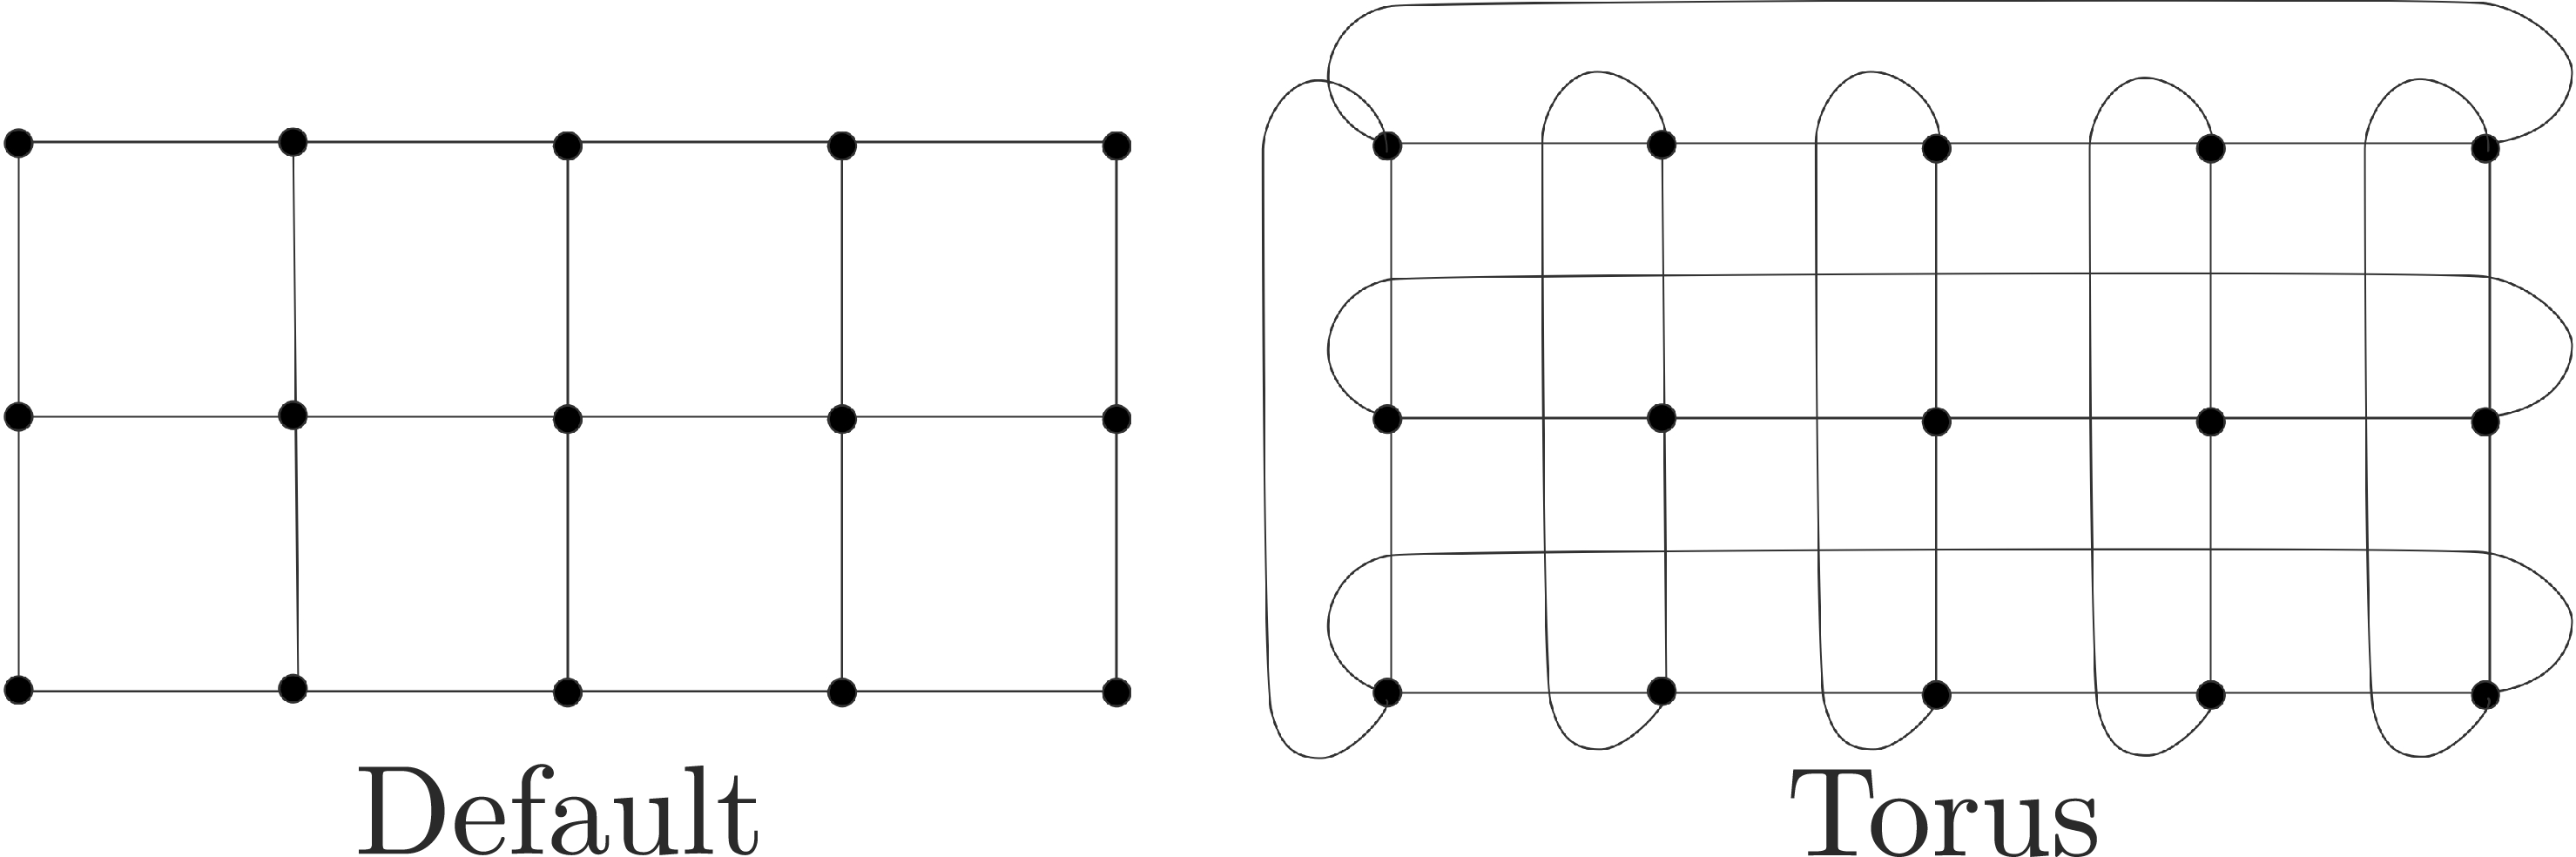
\includegraphics[width=\linewidth]{wrapmode.png}
    \caption{Voisinage des cellules selon le "\texttt{WrapMode}"}
\end{figure}

\pagebreak
\subsection{Classes d'extensions}
\subsubsection{Classe \texttt{ColorExtensions}}
La classe \texttt{ColorExtensions} à pour but de faciliter la conversion entre les objets \texttt{System.Media.Color} utilisé par \textit{LiveCharts} et \texttt{System.Drawing.Color} utilisé par le reste de l'interface graphique et les cellules. Le seul moyen de passer d'un \texttt{System.Drawing.Color} à un \texttt{System.Media.Color} est de convertir la couleur au format hexadécimal. Pour ceci, plusieurs méthodes ont été réalisées : 

\begin{itemize}
    \item \texttt{ToHex(this Color c)}
    \item \texttt{ToHex(this Color c, byte transparency)}
\end{itemize}

La méthode \texttt{ToHex()} permet de convertir une couleur au format hexadécimal. Une surcharge de cette fonction permet de passer en paramètre la transparence désirée. Par exemple, pour récupérer le code hexadécimal de la couleur d'une des stratégies à environ 20\% d'opacité, on peut appeler la fonction de la manière suivante :

\begin{lstlisting}
string result = strategy.getColor().ToHex(51);
\end{lstlisting}

Il donc garder en tête que la transparence est codée sur un seul \textit{byte} (0-255) lors de l'utilisation de la fonction.

\subsubsection{Classe \texttt{ComboBoxExtensions}}
La classe \texttt{ComboBoxExtensions} a été développée dans le but de rendre le choix de la stratégie par l'utilisateur plus agréable. La méthode \texttt{AddStrategies()} permet d'ajouter des stratégies à l'intérieur d'un composant \texttt{ComboBox} à partir d'une liste de stratégies. L'usage standard de cette fonction ressemblerait à :
\begin{lstlisting}
List<Strategy> availableStrategies = new List<Strategy>
availableStrategies.Add(new StratTitForTat());
[...]
comboBox.AddStrategies(availableStrategies);
\end{lstlisting}

La méthode \texttt{DrawItem()} des \texttt{ComboBox} est remplacée par une version ajoutant un rectangle de couleur à coté de chaque élément de la liste. Ceci permet de voir à l'avance les couleurs des cellules placées sur la grille, et d'associer plus facilement une couleur à une stratégie dans l'esprit de l'utilisateur.

\subsection{Classe \texttt{ArrayExtensions}}
La classe \texttt{ArrayExtensions} existe pour faciliter la conversions en différents types de tableaux; principalement, d'un tableau multidimensionnel à un liste et \textit{vice versa}.

Voici les prototypes des fonctions de la classe \texttt{ArrayExtensions} : 

\begin{lstlisting}
// Converts a 2d array to a list.
public static List<object> asList(this object[,] inputArray)

// Converts a list to a 2d array.
public static object[,] asArrayOfArray(this List<object> inputArray, int nbLines, int nbCols)
\end{lstlisting}

Voici un exemple d'utilisation de ces fonctions :
\begin{lstlisting}
Cell[,] cellArray = new Cell[10, 10];
List<Cell> cellList = cellArray.asList();            // Converts to a list
[...]
Cell[,] cellArray2 = cellList.asArrayOfArray(10, 10) // Converts to a 2d array
\end{lstlisting}

\pagebreak
\subsection{Stratégies}
Certaines stratégies connues du dilemme du prisonnier doivent être adaptées avant leur utilisation dans l'automate cellulaire. Les cellules jouent simultanément avec plusieurs voisins mais une seule action est choisie par tour. Cette contrainte nous force à ajuster certaines stratégies.

Dans ce chapitre, le fonctionnement interne de diverses stratégies sera décrit.

\subsubsection{Stratégies simples}
On classifie de stratégies simples les stratégies n'ayant pas besoin de tirer d'informations de l'état du jeu actuel. Des exemples de stratégies simples pourraient être \textit{always cooperate}, \textit{always defect} ou encore \textit{blinker}.

Ces stratégies sont la plupart du temps implémentées en quelques lignes, en voici des exemples :

\begin{lstlisting}
// Blinker
if (cell.History.Count \% 2 == 0)
     { result = Move.Cooperate; }
else { result = Move.Defect; }

return result;

// Always cooperate
return Move.Cooperate;

// Always defect
return Move.Defect;
\end{lstlisting}

\subsubsection{\textit{Tit-for-tat}}
On peut résumer \textit{tit-for-tat} à une stratégie imitant la dernière action de son adversaire. Dans le cas de l'automate cellulaire, une cellule possède plusieurs adversaires ce qui pose un problème : quel adversaire doit-on imiter ?

Dans cette implémentation de \textit{tit-for-tat}, on choisit l'adversaire selon son score. L'adversaire ayant eu le meilleur résultat sera imité. Cette approche est tirée de l'un des travaux étudiés dans l'étude d'opportunité, et se base sur le concept de "\textit{immitation of the best}".

Voici le code de la fonction \texttt{chooseMove()} de \textit{tit-for-tat} :

\begin{lstlisting}
public override Move chooseMove(Cell cell, List<Cell> neighbors)
{
    // Cooperates on first move, then copies his best openent
    Move result = Move.Cooperate;


    // If this wasn't our first round, we look at our neighbors
    if (cell.History.Count > 1)
    {
        // We initialise our variables with the first neighbor in the list
        result = neighbors[0].History.First();
        int min = neighbors[0].Score;

        foreach (Cell neighbor in neighbors)
        {
            if (min > neighbor.Score)
            {
                min = neighbor.Score;
                result = neighbor.History.First();
            }
        }
    }

    return result;
}
\end{lstlisting}

Notez que ce concept est appliqué à toutes les variantes de \textit{tit-for-tat} de l'application.

\pagebreak{}
\subsubsection{\textit{Grim trigger}}
\textit{Grim trigger} est une stratégie coopérant toujours avant d'avoir d'être trahi. Après être trahi, elle trahi tout le temps similaire à \textit{always defect}. Pour illustrer ce principe de mémoire, un booléen est présent dans la classe garde en mémoire si la cellule à été trahie. Ceci est un bon exemple de la flexibilité de la structure, une classe peut avoir des champs et des fonctions a part et peut être considérée comme stratégie si elle implémente \texttt{chooseMove()} et \texttt{getColor()}.

Voici le code de \texttt{chooseMove()} dans cette stratégie :
\begin{lstlisting}
public override Move chooseMove(Cell cell, List<Cell> neighbors)
{
    // Starts by cooperating
    Move result = Move.Cooperate;

    // Check if we were betrayed in the past
    if (WasBetrayed)
    {
        result = Move.Defect;
    }
    else
    {
        // If we didn't get betrayed yet, we look at our neighbors
        if (cell.History.Count > 1)
        {
            // Look if we got betrayed by a neighbor after our first move
            foreach (Cell neighbor in neighbors)
            {
                if (neighbor.History.First() == Move.Defect)
                {
                    // If we are betrayed, we switch to a "Always Defect" strategy
                    this.WasBetrayed = true;
                    result = Move.Defect;
                    break;
                }
            }
        }
    }

    return result;
}
\end{lstlisting}

\pagebreak
\subsection{\textit{Benchmark} des stratégies}
Dans le but de trouver la meilleure stratégie, une partie de l'application permettant de tester les performances d'une stratégie à été réalisée. Depuis cette interface, l'utilisateur peut sélectionner une stratégie à tester, ainsi que le nombre de tours du dilemme du prisonnier à jouer. 

L'inspiration pour cette fonctionnalité provient des tournois du dilemme du prisonnier organisés par Robert Axelrod (popularisés dans son livre : \textit{The Evolution of Cooperation}\cite{book}). Ces tournois ont étés utilisés précédemment dans le but d'analyser les différentes stratégies, leurs performances, ainsi que les critères nécessaires pour qu'une stratégie soit efficace.

Quand l'utilisateur lance la simulation, la stratégie est testée contre toutes les autres stratégies de l'application. La stratégie sélectionnée joue le nombre de parties défini par l'utilisateur contre chacune des stratégies.

Après la simulation terminée, l'utilisateur peut observer les résultats sur un graphique. Le score total de chaque parties contre chaque stratégies est représentée par un histogramme.

\begin{figure}[htp]
    \centering
    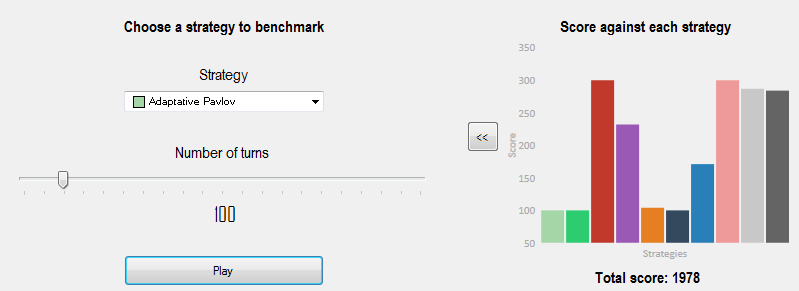
\includegraphics[width=\linewidth - 3cm]{benchmark_gui.png}
    \caption{Interface \textit{benchmark}}
\end{figure}

Grâce à cette fonctionnalité, un graphique démontrant l'efficacité de chaque stratégies à été réalisé. Ce graphique fut réalisé en comparant chaque stratégie sur 100 tours du dilemme du prisonnier. Le score représente le nombre de jours passés en prison, le score le plus bas est donc le meilleur.

\begin{figure}[htp]
    \centering
    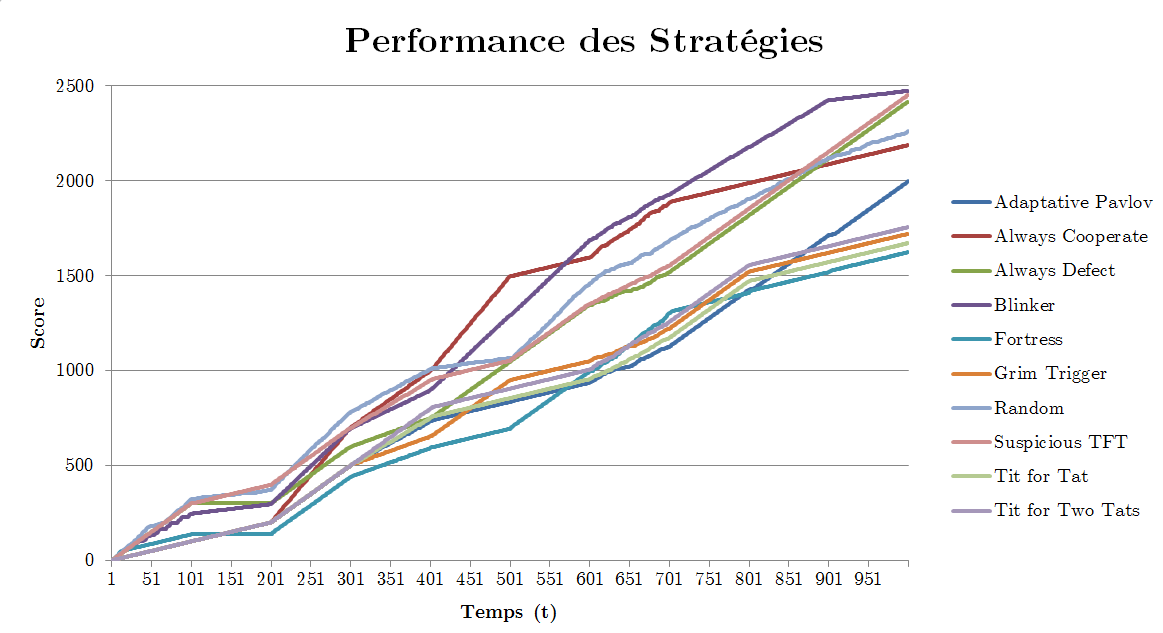
\includegraphics[width=\linewidth - 3cm]{benchmark.png}
    \caption{Test des performances des stratégies}
\end{figure}

\pagebreak
\section{Tests}
Tous les tests unitaires ont étés réalisés dans l'environnement de test de Visual Studio 2013. Cependant, il est actuellement impossible d'exporter les résultats de ces derniers depuis Visual Studio. Pour remédier à ce problème, j'ai développé un script \textit{batch} permettant d'exporter les tests d'une solution au format "\textit{.trx}"\footnote{"\textit{.trx}" représente un fichier de tests crée par Visual Studio} à l'aide de la console de test Visual Studio (vstest.console.exe).

On lance simplement la console de test Visual Studio avec le lien vers notre fichier "\textit{.dll}" de tests et "/Logger:trx" en paramètre. Les résultats seront automatiquement exportés vers un dossier nommé "TestsResults".

Voici le contenu du script \textit{batch} permettant d'exporter les résultat des tests :

\begin{lstlisting}
"C:\[...]\vstest.console.exe" "C:\[...]\PrisonersDilemmaCATests.dll" /Logger:trx
pause
\end{lstlisting}

\vspace{1cm}
\begin{center}
Voici les résultats des tests unitaires des classes de l'automate du cellulaire :
\end{center}
\begin{table}[htp]
\centering
\begin{tabular}{lll}
\hline
\textbf{Nom du test}                        & \textbf{Durée}   & \textbf{Résultat} \\ \hline
CellTests.ConvenianceConstructorTest         & 00:00:00.0002014 & Réussite \\
CellTests.DesignatedConstructorTest          & 00:00:00.0083494 & Réussite \\
CellTests.ImplicitConversionTest             & 00:00:00.0002080 & Réussite \\
CellTests.onClickTest                        & 00:00:00.0060866 & Réussite \\
ColorExtensionsTests.ToHexTest               & 00:00:00.0004385 & Réussite \\
ColorExtensionsTests.ToHexTransparentTest    & 00:00:00.0004142 & Réussite \\
ColorExtensionsTests.ToRGBTest               & 00:00:00.0003641 & Réussite \\
ComboBoxExtensionsTests.AddStrategiesTest    & 00:00:00.0247826 & Réussite \\
GridTests.DesignatedConstructorTest          & 00:00:00.0006595 & Réussite \\
GridTests.findCellNeighborsTest              & 00:00:00.0009470 & Réussite \\
GridTests.getCellTest                        & 00:00:00.0005589 & Réussite \\
GridTests.getPointClampedInGridTest          & 00:00:00.0005565 & Réussite \\
PayoffMatrixTests.DesignatedConstructorTest  & 00:00:00.0002266 & Réussite \\
PayoffMatrixTests.isValidConvenianceTest     & 00:00:00.0003449 & Réussite \\
PayoffMatrixTests.isValidStaticTest          & 00:00:00.0010773 & Réussite \\
PayoffMatrixTests.returnPayoffTest           & 00:00:00.0002335 & Réussite \\
StratAlwaysCooperateTests.chooseMoveTest     & 00:00:00.0004451 & Réussite \\
StratAlwaysDefectTests.chooseMoveTest        & 00:00:00.0004544 & Réussite \\
StratBlinkerTests.chooseMoveTest             & 00:00:00.0011629 & Réussite \\
StrategyTests.CompareToTest                  & 00:00:00.0004379 & Réussite \\
StrategyTests.ToStringTest                   & 00:00:00.0004382 & Réussite \\
StratFortressTests.chooseMoveTest            & 00:00:00.0028304 & Réussite \\
StratGrimTriggerTests.chooseMoveTest         & 00:00:00.0013625 & Réussite \\
StratRandomTests.chooseMoveTest              & 00:00:00.0003097 & Réussite \\
StratSuspiciousTitForTatTests.chooseMoveTest & 00:00:00.0029031 & Réussite \\
StratTitForTatTests.chooseMoveTest           & 00:00:00.0009945 & Réussite \\
StratTitForTwoTatsTests.chooseMoveTest       & 00:00:00.0015303 & Réussite \\
\hline
\end{tabular}
\caption{Résultat des tests unitaires}
\end{table}
\vfill{}

\pagebreak
\section{Estimation de l'apport personnel}
\begin{table}[htp]
\centering
\begin{tabular}{lll}
\hline
\textbf{Nom}        & \textbf{Pourcent} & \textbf{Commentaire}                                      \\ \hline
Grille              & 100\%             &                                                           \\
Cellules            & 100\%             &                                                           \\
Matrice des gains   & 100\%             &                                                           \\
Stratégies          & 100\%             & Implémentation sur la base de courtes descriptions \cite{StratIPD}\cite{StratIPD2}\\
Classes d'extensions& 70\%              & Modification d'algorithmes                                \\
Interface graphique & 90\%              & Utilisation d'une ".dll" pour le composant "ToggleSwitch" \\
Graphiques          & 25\%              & Utilisation de la bibliothèque "LiveCharts"               \\
Tests unitaires     & 100\%             &                                                           \\
Poster              & 100\%             &                                                           \\
Documentation       & 100\%             &                                                           \\ \hline
\end{tabular}
\caption{Apports personnel dans l'automate cellulaire du dilemme du prisonnier}
\end{table}

\section{Conclusions et perspectives}
\subsection{Projet}
En conclusion, le cahier des charges à été entièrement rempli. De plus, quelques fonctionnalités ont pu être ajoutés. La fonction \textit{benchmark} permet à l'utilisateur de tester une stratégie contre toutes les autres stratégies disponibles, dans l'optique de comparer ses résultats. Il est également possible de changer à tout moment le mode d'interaction des cellules. Deux modes sont disponibles, le mode normal et le mode torique (voir Énumération \texttt{WrapMode}). 

\subsection{Améliorations possibles}
Le projet contient actuellement toutes les fonctions décrites dans le cahier des charges, mais n'est évidemment pas parfait. Plusieurs idées viennent à l'esprit lorsque l'on parle d'améliorations possibles :

\begin{itemize}
    \item Amélioration des performances.
    \begin{itemize}
        \item Graphique de la moyenne des scores.
    \end{itemize}
    
    \item Changement de la logique du projet.
    \begin{itemize}
        \item MVC
        \item Huit choix pour huit voisins.
    \end{itemize}
\end{itemize}


\pagebreak
\subsubsection{Graphique de la moyenne des scores}
Le graphique affichant le score moyen de la cellule stocke actuellement tous les résultats de la partie actuelle, ce qui peut causer des ralentissement dans des parties longues. Pour corriger ce problème il est envisageable de créer un nouvel objet compatible avec le graphique de \textit{LiveCharts}. 

Pour cela, l'objet devrait spécifier la coordonnée "$x$" de chaque point au lieu d'être réparti automatiquement par le composant graphique. Cet objet posséderait donc le score et le numéro du tour ou le score à été prit. Après avoir implémenté cela, il ne resterait plus qu'à fixer un seuil pour le nombre d'éléments maximum a stocker et à retirer les éléments en trop.

\begin{figure}[htp]
    \centering
    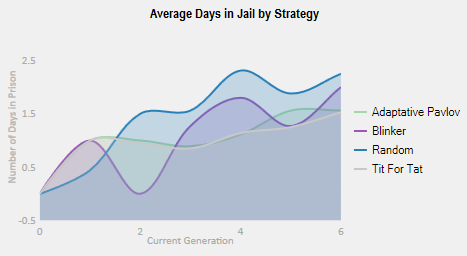
\includegraphics[width=8cm]{graph.png}
    \caption{Graphique causant des problèmes de performances}
\end{figure}

\subsubsection{MVC}
Actuellement le projet utilise une structure de type "\texttt{Model} $\rightarrow{}$ \texttt{View}" ce qui rends plus difficile la séparation du modèle de la vue. Utiliser une architecture MVC simplifierait l'implémentation du modèle dans un autre application.

\subsubsection{Huit choix pour huit voisins}
Actuellement, une seule action est choisi par une cellule, malgré le fait qu'une cellule possède huit voisins au maximum. Ce choix de conception permet de simplifier grandement la logique du jeu malgré les quelques imprécisions qu'elle peut causer au niveau des stratégies. En effet, certaines stratégies ont eu être adaptées pour fonctionner avec l'automate cellulaire. En adoptant une structure ou chaque cellule joue huit parties individuelles avec chacun de ces voisins, les stratégies peuvent rester plus fidèles à leur première implémentation, mais cela au coût de la simplicité. Ce concept pose des problèmes comme "comment définir la couleur de la cellule ?" mais il serait intéressant de l'implémenter pour observer les résultats obtenus.

\pagebreak
\subsection{Évolution de la coopération et fiabilité des stratégies}
Dans "The Evolution of Cooperation" de Robert Axelrod\cite{book}, l'auteur définit différents critères pour qu'une stratégie puisse obtenir un bon score au dilemme du prisonnier. Les critères pour qu'une stratégie soit efficace sont les suivants :

\begin{table}[htp]
\centering
\begin{tabular}{lll}
\hline
\textbf{Anglais}                            & \textbf{}     & \textbf{Français}                          \\ \hline
Don't be envious.                           & $\rightarrow$ & Ne soyez pas envieux.                      \\
Don't be the first to defect.               & $\rightarrow$ & Ne soyez pas le premier a trahir.          \\
Reciprocate both cooperation and defection. & $\rightarrow$ & Réciproquez la coopération et la trahison. \\
Don't be too clever.                        & $\rightarrow$ & Ne soyez pas trop malin.                   \\ \hline
\end{tabular}
\caption{Réussite d'une stratégie}
\end{table}

Le premier critère indique qu'il ne faut pas être envieux, cela implique que la stratégie ne dois pas chercher à avoir le meilleur score de manière égoïste pour réussir.

Le deuxième critère indique qu'il ne faut pas être le premier à trahir ses voisins. Cela assure une relation de "confiance" et empêche certaines stratégies de se "venger" au prochain tour. 

Le troisième critère est qu'il faut réciproquer la trahison et la coopération. En résumé, il est important de coopérer mais il ne faut pas se laisser exploiter par des traîtres et il est nécessaire de trahir si l'adversaire trahit de manière répétée.

Le quatrième critère est qu'il ne faut pas être trop malin. L'auteur fait probablement référence à la stratégie \textit{tit-for-tat} étant l'une des stratégies les plus simples et pourtant la gagnante de plusieurs tournois du dilemme du prisonnier. Ce critère indique aussi que des stratégies plus complexes ne seront pas forcement plus efficaces cela du à la nature du jeu. Une stratégie analysant son adversaire pour déterminer quelle action faire ne sera pas forcement plus efficace qu'une stratégie simple comme \textit{tit-for-tat}.

Dans le cas de l'automate cellulaire du dilemme du prisonnier, ces critères s'appliquent toujours. Cependant, le troisième critère est beaucoup plus difficile à appliquer. Chaque cellule fait un seul choix pour jouer contre ses huit voisins. Cette condition implique que la coopération devient beaucoup plus difficile à rétablir. En effet, si une cellule décide de coopérer, il est nécessaire que la \textit{totalité} de ses voisins coopère pour s'assurer que l'on se fasse pas exploiter par des cellules traîtres. C'est à cause de cette subtilité que des stratégies comme \textit{tit-for-tat} ou \textit{pavlov} ne décident de pas rétablir la coopération.

On peut donc tirer plusieurs conclusions de ces résultats. Du à la nature de l'automate cellulaire, il est difficile de rétablir la coopération après la trahison. De plus, les stratégies simples (\textit{always cooperate}, \textit{blinker}, etc...) ne sont pas une bonne approche et il est nécessaire d'utiliser les informations du plateau pour obtenir de meilleurs scores. Finalement, les stratégies visant à avoir un maximum de points (envieuses) sont plus performantes que dans le dilemme du prisonnier standard (un contre un), cela du à la disposition du jeu (un contre huit) et à la méthode d'attribution des scores (maximisé).

\subsection{Perspectives}
Grâce à ce projet, j'ai pu m'immerger dans un sujet qui m'était inconnu. Il m'aura permit d'appliquer différents concepts appris en classe, tels que : les \textit{design patterns}, le \textit{test driven developpement} ou encore la sérialisation. Il m'a également permit de renforcer mes compétences en documentation avec \LaTeX{}.

Si je venais à travailler à nouveau sur ce projet, je pense changer la structure du programme pour que chaque cellule puisse choisir une action par voisin. 

Finalement, ce projet m'a donné envie de me plonger dans le domaine de la théorie des jeux et de finir la lecture du livre de Robert Axelrod : "L'Évolution de la Coopération".

% End document
\pagebreak
\section{Sources}
\printbibliography{}

\pagebreak
\listoffigures
\listoftables

\pagebreak

% Title page
\pagebreak
\begin{center}
	{\scshape\LARGE CFPT-INFORMATIQUE \par}
	\vspace{0.25cm}
	{\scshape\lesson\par}
	\vspace{3cm}
	
	\hrule
	{\huge\bfseries\textsc{}Code Source\par}
	{\Large\bfseries\textsc\subtitle\par}
	\vspace{0.5cm}
	{\itshape\@author\par}
	\vspace{1cm}
	{\textit{Supervisé par :}  \par \textsc{\teacher}}\par
	\vspace{0.5cm}
	\hrule
	
	\vfill

	\vfill
	\textsc{\class}
	\vspace{1cm}
	
	{\large\today\par}
\end{center}
% End title page
\pagebreak

\section{Code source}
\subsection{Vues}
\subsubsection{AboutView.cs}
\lstinputlisting{code/AboutView.cs}

\subsubsection{GenerateHelpView.cs}
\lstinputlisting{code/GenerateHelpView.cs}

\subsubsection{GenerateView.cs}
\lstinputlisting{code/GenerateView.cs}

\subsubsection{MainView.cs}
\lstinputlisting{code/MainView.cs}

\subsubsection{PayoffMatrixHelpView.cs}
\lstinputlisting{code/PayoffMatrixHelpView.cs}

\subsubsection{PayoffMatrixView.cs}
\lstinputlisting{code/PayoffMatrixView.cs}

\pagebreak
\subsection{Classes}
\subsubsection{Cell.cs}
\lstinputlisting{code/Cell.cs}

\subsubsection{Grid.cs}
\lstinputlisting{code/Grid.cs}

\subsubsection{PayoffMatrix.cs}
\lstinputlisting{code/PayoffMatrix.cs}

\pagebreak
\subsection{Classes d'extensions}
\subsubsection{ArrayExtensions.cs}
\lstinputlisting{code/ArrayExtensions.cs}

\subsubsection{ColorExtensions.cs}
\lstinputlisting{code/ColorExtensions.cs}

\subsubsection{ComboBoxExtensions.cs}
\lstinputlisting{code/ComboBoxExtensions.cs}

\pagebreak
\subsection{Stratégies}
\subsubsection{Strategy.cs}
\lstinputlisting{code/Strategy.cs}

\subsubsection{StratAdaptativePavlov.cs}
\lstinputlisting{code/StratAdaptativePavlov.cs}

\subsubsection{StratAlwaysCooperate.cs}
\lstinputlisting{code/StratAlwaysCooperate.cs}

\subsubsection{StratAlwaysDefect.cs}
\lstinputlisting{code/StratAlwaysDefect.cs}

\subsubsection{StratBlinker.cs}
\lstinputlisting{code/StratBlinker.cs}

\subsubsection{StratFortress.cs}
\lstinputlisting{code/StratFortress.cs}

\subsubsection{StratFortress.cs}
\lstinputlisting{code/StratFortress.cs}

\subsubsection{StratGrimTrigger.cs}
\lstinputlisting{code/StratGrimTrigger.cs}

\subsubsection{StratRandom.cs}
\lstinputlisting{code/StratRandom.cs}

\subsubsection{StratSuspiciousTitForTat.cs}
\lstinputlisting{code/StratSuspiciousTitForTat.cs}

\subsubsection{StratTitForTat.cs}
\lstinputlisting{code/StratTitForTat.cs}

\subsubsection{StratTitForTwoTats.cs}
\lstinputlisting{code/StratTitForTwoTats.cs}

\pagebreak
\subsection{Enums}
\subsubsection{Enums.cs}
\lstinputlisting{code/Enums.cs}

\pagebreak
\subsection{Tests}
\subsubsection{CellTests.cs}
\lstinputlisting{code/tests/CellTests.cs}

\subsubsection{ColorExtensionsTests.cs}
\lstinputlisting{code/tests/ColorExtensionsTests.cs}

\subsubsection{ComboBoxExtensionsTests.cs}
\lstinputlisting{code/tests/ComboBoxExtensionsTests.cs}

\subsubsection{GridTests.cs}
\lstinputlisting{code/tests/GridTests.cs}

\subsubsection{PayoffMatrixTests.cs}
\lstinputlisting{code/tests/PayoffMatrixTests.cs}

\subsubsection{StrategyTests.cs}
\lstinputlisting{code/tests/StrategyTests.cs}

\subsubsection{StratAlwaysCooperateTests.cs}
\lstinputlisting{code/tests/StratAlwaysCooperateTests.cs}

\subsubsection{StratAlwaysDefectTests.cs}
\lstinputlisting{code/tests/StratAlwaysDefectTests.cs}

\subsubsection{StratBlinkerTests.cs}
\lstinputlisting{code/tests/StratBlinkerTests.cs}

\subsubsection{StratFortressTests.cs}
\lstinputlisting{code/tests/StratFortressTests.cs}

\subsubsection{StratGrimTriggerTests.cs}
\lstinputlisting{code/tests/StratGrimTriggerTests.cs}

\subsubsection{StratRandomTests.cs}
\lstinputlisting{code/tests/StratRandomTests.cs}

\subsubsection{StratSuspiciousTitForTatTests.cs}
\lstinputlisting{code/tests/StratSuspiciousTitForTatTests.cs}

\subsubsection{StratTitForTatTests.cs}
\lstinputlisting{code/tests/StratTitForTatTests.cs}

\subsubsection{StratTitForTwoTatsTests.cs}
\lstinputlisting{code/tests/StratTitForTwoTatsTests.cs}
\end{document}